%%%  کلاس AUTthesis، نسخه آبان 1397
%%%   دانشگاه صنعتی امیرکبیر                 http://www.aut.ac.ir
%%%  تالار گفتگوی پارسی‌لاتک،       http://forum.parsilatex.com
%%%   آپدیت شده در آبان 95
%%%   پشتیبانی و راهنمایی          badali_farhad@yahoo.com
%%%
%%%   بازبینی و اصلاح شده در آبان ماه 1397
%%%  Tested via TeXstudio in TeXlive 2014-2018.
%%%

%-----------------------------------------------------------------------------------------------------
%        روش اجرا.: 2 بار F1 ، 2 بار  F11(به منظور تولید مراجع) ، دوبار Ctrl+Alt+I (به منظور تولید نمایه) و دو بار F1 -------> مشاهده Pdf
%%%%%%%%%%%%%%%%%%%%%%%%%%%%%%%%%%%%%%%%%%%%%%%%%%%%%%
%   TeXstudio as your IDE
%%  برای compile در TeXstudio تنها کافی است منوی Options->Configure TeXstudio را زده و در پنجره Configure TeXstudio در بخش Build گزینه Default Compiler را به XeLaTeX تغییر دهید. سند شما به راحتی compile خواهد شد.
%   F1 & F5 : Build & view
%   F6      : Compile
%   F7      : View
%   --------------
%%%%%%%%%%%%%%%%%%%%%%%%%%%%%%%%%%%%%%%%%%%%%%%%%%%%%%
%        اگر قصد نوشتن رساله دکتری را دارید، در خط زیر به جای msc،
%      کلمه phd را قرار دهید. کلیه تنظیمات لازم، به طور خودکار، اعمال می‌شود.
%%% !TEX TS-program = XeLaTeX
\documentclass[oneside,msc,12pt]{AUTthesis}
%       فایل commands.tex را حتماً به دقت مطالعه کنید؛ چون دستورات مربوط به فراخوانی بسته زی‌پرشین 
%       و دیگر بسته‌ها و ... در این فایل قرار دارد و بهتر است که با نحوه استفاده از آنها آشنا شوید. توجه شود برای نسخه نهایی پایان‌نامه حتماً hyperref را 
%        غیرفعال کنید.


% در این فایل، دستورها و تنظیمات مورد نیاز، آورده شده است.
%-------------------------------------------------------------------------------------------------------------------
% در ورژن جدید زی‌پرشین برای تایپ متن‌های ریاضی، این سه بسته، حتماً باید فراخوانی شود.
\usepackage{amsthm,amssymb,amsmath,amsfonts}
% بسته‌ای برای تنطیم حاشیه‌های بالا، پایین، چپ و راست صفحه
\usepackage[top=30mm, bottom=30mm, left=25mm, right=30mm]{geometry}
% بسته‌‌ای برای ظاهر شدن شکل‌ها و تصاویر متن
\usepackage{graphicx}
\usepackage{color}
%بسته‌ای برای تنظیم فاصله عمودی خط‌های متن
\usepackage{setspace}
\usepackage{titletoc}
\usepackage{tocloft}

\usepackage{listings}
\usepackage{color}

\definecolor{dkgreen}{rgb}{0,0.6,0}
\definecolor{gray}{rgb}{0.5,0.5,0.5}
\definecolor{mauve}{rgb}{0.58,0,0.82}

\lstset{frame=tb,
  language=Java,
  aboveskip=3mm,
  belowskip=3mm,
  showstringspaces=false,
  columns=flexible,
  basicstyle={\small\ttfamily},
  numbers=none,
  numberstyle=\tiny\color{gray},
  keywordstyle=\color{blue},
  commentstyle=\color{dkgreen},
  stringstyle=\color{mauve},
  breaklines=true,
  breakatwhitespace=true,
  tabsize=3,
   escapeinside={\%*}{*)},
      morekeywords={encoding,
        xs:schema,xs:element,xs:complexType,xs:sequence,xs:attribute}
}


%با فعال کردن بسته زیر فوت‌نوت‌ها در هر صفحه ریست می‌شوند. حالت پیش‌فرض آن ریست شدن در هر فصل می‌باشد.
%\usepackage[perpage]{footmisc}
\usepackage{enumitem}
%\usepackage{titlesec}
% بسته‌ و دستوراتی برای ایجاد لینک‌های رنگی با امکان جهش
\usepackage[pagebackref=false,colorlinks,linkcolor=blue,citecolor=red]{hyperref}
\usepackage[nameinlink]{cleveref}%capitalize,,noabbrev
 \AtBeginDocument{%
    \crefname{equation}{برابری}{equations}%
    \crefname{chapter}{فصل}{chapters}%
    \crefname{section}{بخش}{sections}%
    \crefname{appendix}{پیوست}{appendices}%
    \crefname{enumi}{مورد}{items}%
    \crefname{footnote}{زیرنویس}{footnotes}%
    \crefname{figure}{شکل}{figures}%
    \crefname{table}{جدول}{tables}%
    \crefname{theorem}{قضیه}{theorems}%
    \crefname{lemma}{لم}{lemmas}%
    \crefname{corollary}{نتیجه}{corollaries}%
    \crefname{proposition}{گزاره}{propositions}%
    \crefname{definition}{تعریف}{definitions}%
    \crefname{result}{نتیجه}{results}%
    \crefname{example}{مثال}{examples}%
    \crefname{remark}{نکته}{remarks}%
    \crefname{note}{یادداشت}{notes}%
}
% چنانچه قصد پرینت گرفتن نوشته خود را دارید، خط بالا را غیرفعال و  از دستور زیر استفاده کنید چون در صورت استفاده از دستور زیر‌‌، 
% لینک‌ها به رنگ سیاه ظاهر خواهند شد که برای پرینت گرفتن، مناسب‌تر است
%\usepackage[pagebackref=false]{hyperref}
% بسته‌ لازم برای تنظیم سربرگ‌ها
\usepackage{fancyhdr}
% بسته‌ای برای ظاهر شدن «مراجع»  در فهرست مطالب
\usepackage[nottoc]{tocbibind}
% دستورات مربوط به ایجاد نمایه
\usepackage{makeidx,multicol}
\setlength{\columnsep}{1.5cm}

%%%%%%%%%%%%%%%%%%%%%%%%%%
\usepackage{verbatim}
\makeindex
\usepackage{sectsty}
% فراخوانی بسته زی‌پرشین و تعریف قلم فارسی و انگلیسی
\usepackage{xepersian}%[extrafootnotefeatures]
\SepMark{-}
%حتماً از تک لایو 2014 استفاده کنید.
\settextfont[Scale=1.3]{B Nazanin}
\setlatintextfont{Georgia}
\renewcommand{\labelitemi}{$\bullet$}
%%%%%%%%%%%%%%%%%%%%%%%%%%
% چنانچه می‌خواهید اعداد در فرمول‌ها، انگلیسی باشد، خط زیر را غیرفعال کنید.
%در غیر اینصورت حتماً فونت PGaramond را نصب کنید.
%\setdigitfont[Scale=1.1]{PGaramond}%%Yas
%%%%%%%%%%%%%%%%%%%%%%%%%%
% تعریف قلم‌های فارسی اضافی برای استفاده در بعضی از قسمت‌های متن
\defpersianfont\nastaliq[Scale=2]{IranNastaliq}
\defpersianfont\chapternumber[Scale=3]{B Nazanin}
%\chapterfont{\centering}%
%%%%%%%%%%%%%%%%%%%%%%%%%%
% دستوری برای تغییر نام کلمه «اثبات» به «برهان»
\renewcommand\proofname{\textbf{برهان}}

% دستوری برای تغییر نام کلمه «کتاب‌نامه» به «منابع و مراجع«
\renewcommand{\bibname}{منابع و مراجع}



% Headings for every page of ToC, LoF and Lot
\setlength{\cftbeforetoctitleskip}{-1.2em}
\setlength{\cftbeforelottitleskip}{-1.2em}
\setlength{\cftbeforeloftitleskip}{-1.2em}
\setlength{\cftaftertoctitleskip}{-1em}
\setlength{\cftafterlottitleskip}{-1em}
\setlength{\cftafterloftitleskip}{-1em}
%%\makeatletter
%%%%\renewcommand{\l@chapter}{\@dottedtocline{1}{1em\bfseries}{1em}}
%%%%\renewcommand{\l@section}{\@dottedtocline{2}{2em}{2em}}
%%%%\renewcommand{\l@subsection}{\@dottedtocline{3}{3em}{3em}}
%%%%\renewcommand{\l@subsubsection}{\@dottedtocline{4}{4em}{4em}}
%%%%\makeatother


\newcommand\tocheading{\par عنوان\hfill صفحه \par}
\newcommand\lofheading{\hspace*{.5cm}\figurename\hfill صفحه \par}
\newcommand\lotheading{\hspace*{.5cm}\tablename\hfill صفحه \par}

\renewcommand{\cftchapleader}{\cftdotfill{\cftdotsep}}
\renewcommand{\cfttoctitlefont}{\hspace*{\fill}\LARGE\bfseries}%\Large
\renewcommand{\cftaftertoctitle}{\hspace*{\fill}}
\renewcommand{\cftlottitlefont}{\hspace*{\fill}\LARGE\bfseries}%\Large
\renewcommand{\cftafterlottitle}{\hspace*{\fill}}
\renewcommand{\cftloftitlefont}{\hspace*{\fill}\LARGE\bfseries}
\renewcommand{\cftafterloftitle}{\hspace*{\fill}}

%%%%%%%%%%%%%%%%%%%%%%%%%%
% تعریف و نحوه ظاهر شدن عنوان قضیه‌ها، تعریف‌ها، مثال‌ها و ...
%برای شماره گذاری سه تایی قضیه ها
\theoremstyle{definition}
\newtheorem{definition}{تعریف}[section]
\newtheorem{remark}[definition]{نکته}
\newtheorem{note}[definition]{یادداشت}
\newtheorem{example}[definition]{نمونه}
\newtheorem{question}[definition]{سوال}
\newtheorem{remember}[definition]{یاداوری}
\theoremstyle{theorem}
\newtheorem{theorem}[definition]{قضیه}
\newtheorem{lemma}[definition]{لم}
\newtheorem{proposition}[definition]{گزاره}
\newtheorem{corollary}[definition]{نتیجه}
%%%%%%%%%%%%%%%%%%%%%%%%
%%%%%%%%%%%%%%%%%%%
%%% برای شماره گذاری چهارتایی قضیه ها و ...
%%\newtheorem{definition1}[subsubsection]{تعریف}
%%\newtheorem{theorem1}[subsubsection]{قضیه}
%%\newtheorem{lemma1}[subsubsection]{لم}
%%\newtheorem{proposition1}[subsubsection]{گزاره}
%%\newtheorem{corollary1}[subsubsection]{نتیجه}
%%\newtheorem{remark1}[subsubsection]{نکته}
%%\newtheorem{example1}[subsubsection]{مثال}
%%\newtheorem{question1}[subsubsection]{سوال}

%%%%%%%%%%%%%%%%%%%%%%%%%%%%

% دستورهایی برای سفارشی کردن صفحات اول فصل‌ها
\makeatletter
\newcommand\mycustomraggedright{%
 \if@RTL\raggedleft%
 \else\raggedright%
 \fi}
\def\@makechapterhead#1{%
\thispagestyle{style1}
\vspace*{20\p@}%
{\parindent \z@ \mycustomraggedright
\ifnum \c@secnumdepth >\m@ne
\if@mainmatter

\bfseries{\Huge \@chapapp}\small\space {\chapternumber\thechapter}
\par\nobreak
\vskip 0\p@
\fi
\fi
\interlinepenalty\@M 
\Huge \bfseries #1\par\nobreak
\vskip 120\p@

}

%\thispagestyle{empty}
\newpage}
\bidi@patchcmd{\@makechapterhead}{\thechapter}{\tartibi{chapter}}{}{}
\bidi@patchcmd{\chaptermark}{\thechapter}{\tartibi{chapter}}{}{}
\makeatother

\pagestyle{fancy}
\renewcommand{\chaptermark}[1]{\markboth{\chaptername~\tartibi{chapter}: #1}{}}

\fancypagestyle{style1}{
\fancyhf{} 
\fancyfoot[c]{\thepage}
\fancyhead[R]{\leftmark}%
\renewcommand{\headrulewidth}{1.2pt}
}


\fancypagestyle{style2}{
\fancyhf{}
\fancyhead[R]{چکیده}
\fancyfoot[C]{\thepage{}}
\renewcommand{\headrulewidth}{1.2pt}
}

\fancypagestyle{style3}{%
  \fancyhf{}%
  \fancyhead[R]{فهرست نمادها}
  \fancyfoot[C]{\thepage}%
  \renewcommand{\headrulewidth}{1.2pt}%
}

\fancypagestyle{style4}{%
  \fancyhf{}%
  \fancyhead[R]{فهرست جداول}
  \fancyfoot[C]{\thepage}%
  \renewcommand{\headrulewidth}{1.2pt}%
}

\fancypagestyle{style5}{%
  \fancyhf{}%
  \fancyhead[R]{فهرست اشکال}
  \fancyfoot[C]{\thepage}%
  \renewcommand{\headrulewidth}{1.2pt}%
}

\fancypagestyle{style6}{%
  \fancyhf{}%
  \fancyhead[R]{فهرست مطالب}
  \fancyfoot[C]{\thepage}%
  \renewcommand{\headrulewidth}{1.2pt}%
}

\fancypagestyle{style7}{%
  \fancyhf{}%
  \fancyhead[R]{نمایه}
  \fancyfoot[C]{\thepage}%
  \renewcommand{\headrulewidth}{1.2pt}%
}

\fancypagestyle{style8}{%
  \fancyhf{}%
  \fancyhead[R]{منابع و مراجع}
  \fancyfoot[C]{\thepage}%
  \renewcommand{\headrulewidth}{1.2pt}%
}
\fancypagestyle{style9}{%
  \fancyhf{}%
  \fancyhead[R]{واژه‌نامه‌ی فارسی به انگلیسی}
  \fancyfoot[C]{\thepage}%
  \renewcommand{\headrulewidth}{1.2pt}%
}
%

%دستور حذف نام لیست تصاویر و لیست جداول از فهرست مطالب
\newcommand*{\BeginNoToc}{%
  \addtocontents{toc}{%
    \edef\protect\SavedTocDepth{\protect\the\protect\value{tocdepth}}%
  }%
  \addtocontents{toc}{%
    \protect\setcounter{tocdepth}{-10}%
  }%
}
\newcommand*{\EndNoToc}{%
  \addtocontents{toc}{%
    \protect\setcounter{tocdepth}{\protect\SavedTocDepth}%
  }%
}
\newcounter{savepage}
\renewcommand{\listfigurename}{فهرست اشکال}
\renewcommand{\listtablename}{فهرست جداول}
\usepackage{booktabs}% http://ctan.org/pkg/booktabs
\newcommand{\tabitem}{~~\llap{\textbullet}~~}
%\renewcommand\cftsecleader{\cftdotfill{\cftdotsep}}
%%%%%%%%%%%%%%%%%%%%%%%%%%%%%
%%%%%%%%%%%%%%%%%%%%%%%%%%%%

\begin{document}
\baselineskip=.75cm
\linespread{1.75}
%% -!TEX root = AUTthesis.tex
% در این فایل، عنوان پایان‌نامه، مشخصات خود، متن تقدیمی‌، ستایش، سپاس‌گزاری و چکیده پایان‌نامه را به فارسی، وارد کنید.
% توجه داشته باشید که جدول حاوی مشخصات پروژه/پایان‌نامه/رساله و همچنین، مشخصات داخل آن، به طور خودکار، درج می‌شود.
%%%%%%%%%%%%%%%%%%%%%%%%%%%%%%%%%%%%
% دانشکده، آموزشکده و یا پژوهشکده  خود را وارد کنید

\faculty{دانشکده مهندسی کامپیوتر و فناوری اطلاعات}
% گرایش و گروه آموزشی خود را وارد کنید
\department{گرایش معماری سیستم‌های کامپیوتری}
% عنوان پایان‌نامه را وارد کنید
\fatitle{طراحی و پیاده‌سازی سامانه اطلاعات کالا در فروشگاه‌ها و انبارها
\\[.75 cm]
}
% نام استاد(ان) راهنما را وارد کنید
\firstsupervisor{دکتر بهادر بخشی سراسکانرود}
%\secondsupervisor{استاد راهنمای دوم}
% نام استاد(دان) مشاور را وارد کنید. چنانچه استاد مشاور ندارید، دستور پایین را غیرفعال کنید.
%\firstadvisor{دکتر حامد فربه}
%\secondadvisor{استاد مشاور دوم}
% نام نویسنده را وارد کنید
\name{امین }
% نام خانوادگی نویسنده را وارد کنید
\surname{رشیدبیگی}
%%%%%%%%%%%%%%%%%%%%%%%%%%%%%%%%%%
\thesisdate{مهر‌ماه 1398}

% چکیده پایان‌نامه را وارد کنید
\fa-abstract{
<<<<<<< HEAD
مدیریت و یافتن کالاها در فروشگاه‌ها و انبار‌های بزرگ یکی از دغدغه‌های فروشندگان و مدیران انبارهاست. هدف این پروژه پیاده‌سازی سیستم سامانه‌ی مدیریت و دریافت اطلاعات کالاها در این محیط‌هاست. این سامانه متشکل از قطعه‌های سخت‌افزاری و همچنین نرم‌افزار لازم برای تعامل با کاربر است. این سامانه از طریق بوردها و صفحه‌های نمایش لمسی قرار گرفته بر روی آنها در قسمت‌ها و دسته‌های مختلف انبار و فروشگاه، این اجازه را به کارکنان انبار و فروشگاه می‌دهد که موجودی کالا‌های خود را به روز‌رسانی کنند و از طریق نرم‌افزار مربوطه، مکان، موجودی و سایر مشخصات کالا را جست‌و‌جو کنند. بوردها این اطلاعات را از طریق یک پایگاه‌داده دریافت می‌کنند و پس از هرگونه عملیات جمع‌آوری، این اطلاعات در پایگاه‌داده بروزرسانی می‌شود. خروجی این سامانه، نرم‌افزاری تحت وب با رابط کاربری مناسب است که محل قرارگیری کالا‌های موجود در انبار و فروشگاه را مشخص می‌کند و قابلیت جست‌و‌جو در بین این کالا‌ها را به کاربر می‌دهد.
=======
مدیریت و یافتن کالاها در فروشگاه‌ها و انبار‌های بزرگ یکی از دغدغه‌های فروشندگان و مدیران انبارهاست. هدف این پروژه پیاده‌سازی سیستم سامانه‌ی مدیریت و دریافت اطلاعات کالاها در این محیط‌هاست. این سامانه متشکل از قطعه‌های سخت‌افزاری و همچنین نرم‌افزار لازم برای تعامل با کاربر است. این سامانه از طریق بوردها و صفحه‌های نمایش لمسی قرار گرفته بر روی آنها در قسمت‌ها و دسته‌های مختلف انبار و فروشگاه، این اجازه را به کارکنان انبار و فروشگاه می‌دهد که موجودی کالا‌های خود را به روز‌رسانی کنند و از طریق نرم‌افزار مربوطه، مکان، موجودی و سایر مشخصات کالا را جست‌و‌جو کنند. بوردها این اطلاعات را از طریق یک پایگاه‌داده دریافت می‌کنند و پس از هرگونه عملیات جمع‌آوری، این اطلاعات در پایگاه‌داده بروزرسانی می‌شود. خروجی این سامانه، نرم‌افزاری تحت وب با رابط کاربری مناسب ‌می‌باشد که محل قرارگیری کالا‌های موجود در انبار و فروشگاه را مشخص می‌کند و قابلیت جست‌و‌جو در بین این کالا‌ها را به کاربر می‌دهد.
>>>>>>> 0b914906bc0a1f3ca7b01ffa78967759bf4780dc
}

% کلمات کلیدی پایان‌نامه را وارد کنید
\keywords{
انبارداری، هوشمند، فروشگاه، کالا
}




\AUTtitle
%%%%%%%%%%%%%%%%%%%%%%%%%%%%%%%%%%
\vspace*{7cm}
\thispagestyle{empty}
\begin{center}

\includegraphics[height=5cm,width=12cm]{besm}
\end{center}
% تاییدیه دفاع
\newpage
\thispagestyle{empty}
%\fontsize{18pt}{19pt}\selectfont

\section*{صفحه فرم ارزیابی و تصویب پایان نامه- فرم تأیید اعضاء كميته دفاع}

\fontsize{12pt}{14pt}\selectfont
%\renewcommand{\baselinestretch}{1.5}
\vspace*{1cm}
   در این صفحه فرم دفاع یا تایید و تصویب پایان نامه موسوم به فرم کمیته دفاع- موجود در پرونده آموزشی- را قرار دهید.
\vspace*{1cm}


\subsection*{نکات مهم:}
 
\begin{itemize}
\item
	نگارش پایان نامه/رساله باید به
	{\color{red}
		زبان فارسی
	}
	و بر اساس آخرین نسخه دستورالعمل و راهنمای تدوین پایان نامه های دانشگاه صنعتی امیرکبیر باشد.(دستورالعمل و راهنمای حاضر)
\item رنگ جلد پایان نامه/رساله چاپي كارشناسي، كارشناسي ارشد و دكترا  بايد به ترتيب مشكي، طوسي و سفيد رنگ باشد.  
\item چاپ و صحافی پایان نامه/رساله بصورت
{\color{red}
	پشت و رو(دورو)
}
بلامانع است و انجام آن توصيه مي شود. 
\end{itemize}
%%%%%%%%%%%%%%%%%%%%%%%%%%%%%%%%%%%%%%%%%%%%%%%%%%%%%%%%%%%%%%%%%%%%%%%%%%%%%%%%%%%%%%%%%%%%%%%%%%
%%%%%%%%%%%%%%%%%%%%%%%%%%%%%%%%%%%%%%%%%%%%%%%%%%%%%%%%%%%%%%%%%%%%%%%%%%%%%%%%%%%%%%%%%%%%%%%%%%
\newpage
\thispagestyle{empty}
\begin{picture}(50,50)
  \put(17,0){
\includegraphics[scale=1.1]{fa-logo}}
  \put(4.5,-13){\footnotesize{دانشگاه صنعتی امیرکبیر}}
  \put(10.5,-27){\footnotesize{(پلی‌تکنیک تهران)}}
  \put(170,30){\bf{به نام خدا}}
  \put(140,-5){\Large\bf{تعهدنامه اصالت اثر}}
  \put(310,0){تاریخ: \datethesis}
\end{picture}

\vspace*{2.5cm}

اينجانب {\bf{\fname\lname}} متعهد می‌شوم که مطالب مندرج در این پایان‌نامه حاصل کار پژوهشی اینجانب تحت نظارت و راهنمایی اساتید دانشگاه صنعتی امیرکبیر بوده و به دستاوردهای دیگران که در این پژوهش از آنها استفاده شده است مطابق مقررات و روال متعارف ارجاع و در فهرست منابع و مآخذ ذکر گردیده است. این پایان‌نامه قبلاً برای احراز هیچ مدرک هم‌سطح یا بالاتر ارائه نگردیده است.

در صورت اثبات تخلف در هر زمان، مدرک تحصیلی صادر شده توسط دانشگاه از درجه اعتبار ساقط بوده و دانشگاه حق پیگیری قانونی خواهد داشت.


کلیه نتایج و حقوق حاصل از این پایان‌نامه متعلق به دانشگاه صنعتی امیرکبیر می‌باشد. هرگونه استفاده از نتایج علمی و عملی، واگذاری اطلاعات به دیگران یا چاپ و تکثیر، نسخه‌برداری، ترجمه و اقتباس از این پایان نامه بدون موافقت کتبی دانشگاه صنعتی امیرکبیر ممنوع است. 
نقل مطالب با ذکر مآخذ بلامانع است.\\
\vspace{2.5cm}


{\centerline {\bf{\fname\lname}}}
\vspace*{.2cm}
{\centerline{امضا}}
%%%%%%%%%%%%%%%%%%%%%%%%%%%%%%%%%
% چنانچه مایل به چاپ صفحات «تقدیم»، «نیایش» و «سپاس‌گزاری» در خروجی نیستید، خط‌های زیر را با گذاشتن ٪  در ابتدای آنها غیرفعال کنید.
% پایان‌نامه خود را تقدیم کنید
% نیایش خود را در فایل زیر بنویسید.
\begin{acknowledgementpage}

\vspace{1.5cm}

{\nastaliq
{
تقدیم به \\
خالق بی‌نهایت‌ها،\\
پرسشگران خلاق، \\
و غواصان خستگی‌ناپذیر دریای پاسخ‌ها.\\
}}\end{acknowledgementpage}
\newpage
% سپاسگزاری را در فایل زیر بنویسید.
%%%%%%%%%%%%%%%%%%%%%%%%%%%%%%%%%%%%
\newpage\thispagestyle{empty}
% سپاس‌گزاری
{\nastaliq
سپاس‌گزاری
}
\\[2cm]

 از پدرم که چون کوهی استوار و مادرم که چون دریای محبت در فراز و نشیب زندگی دلسوزانه همراهم بوده‌اند؛\\
 از اساتید بزرگوار جناب آقای دکتر بهادر بخشی که در کمال سعه صدر، با حسن خلق و فروتنی، رهنمون من شده‌اند؛\\
و از سایر عزیزانی که در کنارشان این نتیحه حاصل آمد کمال تشکر و قدردانی را دارم.

\signature








%%%%%%%%%%%%%%%%%%%%%%%%%%%%%%%%%%%%%%%%%
%%%%%%%%%%%%%%%%%%%%%%%%%%%%%%%%%کدهای زیر را تغییر ندهید.
\newpage\clearpage

\pagestyle{style2}

\vspace*{-1cm}
\section*{\centering چکیده}
%\addcontentsline{toc}{chapter}{چکیده}
\vspace*{.5cm}
\ffa-abstract
\vspace*{2cm}


{\noindent\large\textbf{واژه‌های کلیدی:}}\par
\vspace*{.5cm}
\fkeywords
% دستور زیر برای شماره گذاری صفحات قبل از فصل اول با حروف ابجد است.
\pagenumbering{alph}
%-----------------------------------------------------------------------------
% فایل زیر دستورات مربوط به نمایش صفحات فهرست مطالب- فهرست اشکال و جداول است.
%{\pagestyle{style2}
%\tableofcontents}\newpage
%
%\listoffigures
\cleardoublepage
\pagestyle{style6}
\tableofcontents
\pagestyle{style6}
\cleardoublepage
%اگر لیست تصاویر و لیست جداول ندارید ، کدهای زیر را با گذاشتن % در ابتدای آنها، غیرفعال کنید.
\BeginNoToc
%============
\addtocontents{lof}{\lofheading}% add heading to the first page in LoF
\pagestyle{style5}
\listoffigures
\thispagestyle{style5}
\cleardoublepage
%============
\addtocontents{lot}{\lotheading}% add heading to the first page in LoT
\thispagestyle{style4}
%\listoftables
\thispagestyle{style4}
%============
%\cleardoublepage
%
\cleardoublepage
\setcounter{savepage}{\arabic{page}}
\mainmatter
\addtocontents{toc}{\tocheading}% add heading to the first page in ToC, after frontmatter entries
\EndNoToc
% در صورت تمایل می‌توانید با فعال کردن دستور بالا، لیست تصاویر را به  پایان‌نامه خود اضافه کنید.
%-------------------------------------------------------------------------symbols(فهرست نمادها)
% وجود لیست نمادها الزامیست.(لطفاً نمادهای خود را جایگذین نمادهای پیش‌فرض کنید.)
%%%%%%%%%%%%%

{\centering\LARGE\textbf{فهرست نمادها}\par}%

\pagenumbering{alph}
\setcounter{page}{\thesavepage}
%\setcounter{page}{6}
\vspace*{1cm}

\pagestyle{style3}
%\thispagestyle{empty}
%\addcontentsline{toc}{chapter}{فهرست نمادها}
\symb{\text{ نماد}}{مفهوم}
\\
%مقادیر بالا را تغییر ندهید
%%%%%%%%%%%%%%%%%%%%%%%%%%%%%%%%%%%%%%%%%%%%%%%%%%%%%%%%%
\symb{\mathbb{R}^n}{
فضای اقلیدسی با بعد $n$
}
\symb{\mathbb{S}^n}{
کره یکه $n$ بعدی
}
\symb{M^m}{
خمینه $m$-بعدی $M$
}
\symb{\mathfrak{X}(M)}{
جبر میدان‌های  برداری هموار روی $M$
}
\symb{\mathfrak{X}^1(M)}{
مجموعه میدان‌های برداری هموار یکه روی $(M,g)$ 
}
\symb{\Omega^p(M)}{
مجموعه $p$-فرمی‌های روی خمینه $M$
}
\symb{Q}{
اپراتور ریچی
}
\symb{\mathcal{R}}{
تانسور انحنای ریمان
}
\symb{ric}{
تانسور ریچی
}
\symb{L}{
مشتق لی
}
\symb{\Phi}{
2-فرم اساسی خمینه تماسی
}
\symb{\nabla}{
التصاق لوی-چویتای
}
\symb{\Delta}{
لاپلاسین ناهموار
}
\symb{\nabla^*}{
عملگر خودالحاق صوری القا شده از التصاق لوی-چویتای
}
\symb{g_s}{
متر ساساکی
}
\symb{\nabla}{
التصاق لوی-چویتای وابسته به متر ساساکی
}
\symb{\Delta}{
عملگر لاپلاس-بلترامی روی $p$-فرم‌ها
}

%%%%%%%%%%%%%%%%%%%%%%%%%%%%%%%%%%%%%%%

\thispagestyle{style3}
\newpage
%\pagestyle{style1}
%%%%%%%%%%%%%%%%%%%%%%%%%%%%%%%%%%%%


\pagenumbering{arabic}
\pagestyle{style1}
%--------------------------------------------------------------------------chapters(فصل ها)
\chapter{مقدمه}
\section{مقدمه}
انبارها ساختمان یا محوطه‌ای هستند که برای نگهداری کالاها استفاده می‌گردند. صنعت‌گران، واردکنندگان، صادرکنندگان، عمده‌فروشان و گمرک، استفاده‌کنندگان انبارها می‌باشند. انبارها معمولاً در شهرها، شهرک‌های صنعتی و کارخانجات ساخته می‌شوند ولی ممکن است جهت سهولت در دریافت و صدور کالا، در کنار راه‌های اصلی، فرودگاه و یا بنادر نیز ساخته شوند تا کالاها مستقیماً به آنجا وارد و یا خارج گردد.

انبار‌ها از لحاظ کاربری ممکن است انواع گوناگونی داشته باشند. انبار محصول، انبار مواد اولیه، انبار قطعات نیم‌سوخته، انبار قطعات یدکی، انبار ابزار آلات، انبار غلات و مخازن تنها تعداد اندکی از انواع انبارها می‌باشند. با توجه به کاربری و تنوع زیاد انواع انبارها، ماشین آلات، سیستم‌ها و تجهیزات سخت‌افزاری و نرم‌افزاری بسیاری متناسب با نوع کاربری انبارها توسعه یافته‌اند. از آنجا که انبارها در فرآیند تجارت هیچ‌گونه ارزش افزوده‌ای ایجاد نمی‌نمایند، مکان‌یابی، جابجایی و خروج کالاها از انبار بسیار خطیر است و لازم است تا عملیات انبارها با حداقل هزینه و حداکثر بهره‌وری انجام پذیرد.

سیستم اداره انبارها با توجه به نوع کاربری و جامعه مورد استفاده بسیار متفاوت است. در برخی از جوامع، انبارها هنوز به صورت سنتی اداره می‌گردند، حال آنکه برخی از انبارها کاملاً خودکار و مکانیزه می‌باشند؛ بدون اینکه نیاز به نیروی کار انسانی داشته باشند و از طریق سیستم‌های دریافت و انتقال خودکار کالاها و نرم افزارهای لجستیکی\LTRfootnote{\lr{Logistic}} مدیریت می‌شوند.

انبارداری به صورت سنتی، در صورت افزایش مقیاس انبار، مشکلات زیادی را به وجود می‌آورد. در این روش هرگونه مشکل پیش‌آمده برای کارکنان انبار باعث ضرر و زیان مالی می‌شود. از این مشکلات می‌توان به خستگی، چندکاری، محیط پر سروصدا و کاهش تمرکز کارکنان اشاره کرد.
 
 
مشکل پیدا کردن و جمع‌آوری کالاهای مورد نیاز در فروشگاه‌ها و انبارهای بزرگ، همواره دغدغه کارخانه‌ها و شرکت‌های توزیع‌کننده و صاحبان فروشگاه‌ها بوده‌است. این مشکل زمانی حیاتی می‌شود که جایگاه کالاها ثابت نباشد و در طول زمان تغییر کند. در این صورت جمع‌آوری کالا به گلوگاه مجموعه تبدیل می‌شود. در در جامعه کنونی و در شرایط فعلی، این روندها بیشتر به صورت انسانی و بدون کمک رایانه انجام می‌شوند. از موارد مشکل‌ساز روند فعلی، می‌توان به افزایش هزینه‌های چیدمان و نگهداری کالاها اشاره کرد. چون چیدمان نامناسب کالاها و جمع‌آوری آن‌ها در انبارها، به نیروی انسانی بیشتری نیاز دارد.
 
این پروژه، امکانی را برای کارکنان فراهم می‌کند که جایگاه اجناس را به وسیله قطعه‌های سخت افزاری بروزرسانی کنند و همچنین نرم‌افزاری در اختیار آنان قرار می‌دهد تا به وسیله آن، بتوانند بسیار راحت‌تر و سریع‌تر موارد مورد نیاز خود را پیدا کنند. همچنین این پروژه به مشتریان فروشگاه‌های بزرگ و زنجیره‌ای کمک می‌کند که اطلاعات و جایگاه کالاهای موجود در لیست خریدشان را دریافت کنند. علاوه بر این، رابطی برای مدیریت مجموعه فراهم شده‌است تا بتوانند وضعیت فعلی مجموعه را زیر نظر داشته باشند و در صورت نیاز، تغییراتی در سیستم اعمال کنند.
 
در این نوشته، ابتدا به تعریف مسئله و راه حل پیشنهادی و همچنین نیازمندی‌های مسئله پرداخته می‌شود. سپس تکنولوژی‌های نرم‌افزاری و همچنین قطعات سخت‌افزاری انتخاب شده معرفی می‌گردند. در قسمت بعد به شرح مفصل پیاده‌سازی راه‌حل پرداخته می‌شود و در نهایت به جمع‌بندی کارهای انجام شده و همچنین کارهایی که در آینده برای این پروژه می‌توان انجام داد پرداخته می‌شود.
\chapter{تعریف مسئله، راه حل پیشنهادی و تعریف نیازمندی‌ها}
\section{مقدمه}
در این قسمت ابتدا به تعریف و طرح مسئله پرداخته می‌شود. سپس راه‌حلی پیشنهاد داده می‌شود و در ادامه نیازمندی‌های پروژه بر اساس راه حل پیشنهادی تعریف می‌شود.
پیش از آغاز پیاده‌سازی نرم‌افزار لازم است درک جامع و کاملی از مسئله پیدا کنیم و فهرست دقیقی از نیازمندی‌های آن تهیه نماییم. در این فصل سعی شده است پس از بیان مسئله، نیازمندی‌ها و روش حل آن مشخص شوند.

\section{تعریف مسئله}
مدیریت و یافتن کالاها در فروشگاه‌ها و انبار‌های بزرگ، یکی از دغدغه‌های اصلی فروشندگان و انباردارهاست. هنگامی که سفارشی ثبت می‌شود، جمع‌آورنگان محصولات در انبارها وظیفه دارند در انبوهی از کالاها و بخش‌های انبار، کالاهای ثبت‌شده در سفارش را جمع‌آوری کنند. اگر انبار مربوطه تعداد زیادی کالا داشته باشد و یا انباری مربوط به کسب‌و‌کارهایی با محصولات پرمصرف باشد، این موضوع به گلوگاه تبدیل می‌شود. همچنین مشتریان فروشگاه‌های زنجیره‌ای همواره با پیدا کردن لیست محصولات مورد نیاز خود در بین انبوهی از کالاها مشکل دارند. کاهش زمان صرف‌شده برای جمع‌آوری کالاها، برای مدیران 
انبارها، از اهمیت ویژه‌ای برخوردار است.


\section{راه حل پیشنهادی} 
راه حل پیشنهادی برای حل این مسئله، طراحی و پیاده‌سازی سامانه‌ای جهت مدیریت، ایجاد تغییرات و کنترل کالاها در جایگاه‌های متفاوت در این محیط‌هاست. این سامانه متشکل از قطعه‌های سخت‌افزاری و همچنین نرم‌افزار لازم برای تعامل با کاربر است. این سامانه از طریق بوردها و صفحه‌های نمایش لمسی قرار گرفته بر روی آن، در قسمت‌ها و دسته‌های مختلف انبار و فروشگاه، این اجازه را به کارکنان انبارها و فروشگاه‌ها می‌دهد که موجودی کالا‌های خود را به روز‌رسانی کنند و از طریق نرم‌افزار مربوطه، مکان، موجودی و سایر مشخصات کالا را جست‌و‌جو کنند. همچنین به یک برنامه سمت کاربر جهت مدیریت داده‌ها و کاربران نیاز است.


\section{نیازمندی‌های پروژه}
با توجه به موارد مطرح شده در قسمت تعریف مسئله و همچنین در قسمت راه حل پیشنهادی، نیازمندی‌هایی به وجود آمد که در ادامه به آن‌ها پرداخته می‌شود.

\subsection{رابط کاربری مدیریت}
پروژه شامل کاربرها و محصولات، بخش‌ها\LTRfootnote{\lr{Segments}}، سفارش‌ها و دسته‌بندی‌های مختلف است. برای مدیریت و کنترل این قسمت‌ها، به یک محیطی نیاز است که مدیر، دسترسی تغییر بخش‌های مختلف را بر اساس نیاز داشته باشد.

مدیر در محیط مدیریت\LTRfootnote{\lr{Admin Panel}} باید بتواند اعمال زیر را انجام دهد:
\begin{itemize}
   	\item اضافه کردن، ویرایش و یا حذف یک محصول
   	\item اضافه کردن، ویرایش و یا حذف یک دسته‌بندی
   	\item اضافه کردن، ویرایش و یا حذف یک بخش
   	\item مشاهده و ویرایش سفارش‌های ثبت شده
\end{itemize}
با توجه به این که ممکن است بر اساس نیاز، لازم شود افراد دیگری غیر از مدیر اصلی توانایی تغییر بخش‌های ذکر شده را داشته باشند، باید امکانِ دادن دسترسی به کاربران دیگر نیز داده شود. همچنین نیاز است سطح دسترسی کاربران تحت عنوان نقش‌های مختلف نیز تعریف شوند. از وظایف مدیر اصلی رابط کاربری مدیریت، تعیین دسترسی‌های کاربران و نقش‌های مختلف برنامه است.

\subsection{برنامه جمع‌آوری محصولات سفارش‌ها}
جمع‌آورندگان\LTRfootnote{\lr{Picker}} داخل انبار و فروشگاه نیاز دارند تا از سفارش‌های ثبت شده مطلع شوند تا به جمع‌آوری محصولات آن سفارش بپردازند. همچنین پس از جمع‌آوری محصولات، به مدیر و بقیه جمع‌آورندگان باید اطلاع دهند که سفارش جمع‌آوری گردید.

این برنامه شامل موارد زیر است:
\begin{itemize}
	\item مشاهده سفارش‌های ثبت شده و وضعیت آن‌ها
	\item مشاهده محصولات سفارش
	\item اطلاع‌ دادن پس از جمع‌آوری محصولات سفارش
\end{itemize}

\subsection{برنامه انتخاب محصولات بخش‌ها‌}
بخش‌های مختلف در انبارها و فروشگاه‌ها دارای محصولات متفاوتی هستند. این محصولات در طول زمان اضافه، کم ویا جابجا می‌شوند.

در این پروژه به قطعات سخت‌افزاری جهت قرارگیری بر روی بخش‌های مختلف نیاز است تا کاربر بتواند به راحتی با آن تعامل برقرار کند و محصولات فعلی بخش  و موجودی آن‌ها را ثبت کنند. برای ثبت محصولات، علاوه بر قطعات سخت‌افزاری، به برنامه‌ای نیاز است تا محصولات موجود را نمایش دهد و پس از تغییر جایگاه محصولات، آن تغییر را در پایگاه‌داده ثبت کند.

\section{نتیجه‌گیری}
در این قسمت مسئله مورد نظر تعریف و شرح داده شد. همچنین راه‌حلی پیشنهادی برای مسئله ارائه شد. در نهایت و با توجه به راه حل، نیازمندی‌های مسئله تعریف شد. این نیازمندی‌ها شامل برنامه‌های سمت کاربر و همچنین مدیریت مجموعه است.

\chapter{اجزا و تکنولوژی‌ها}
%\thispagestyle{empty}

\section{مقدمه}
در این قسمت اجزا، قطعات و تکنولوژی‌های سخت‌افزای و نرم‌افزاری مورد استفاده در پروژه معرفی خواهند شد.

\section{رزبری‌پای مدل \lr{3A}}
امروزه با پیشرفت روزافزون تکنولوژی و ظهور پردازنده‌های کم‌مصرف آرم\LTRfootnote{\lr{ARM}}، حجم و وزن کامپیوترها هرروز کوچک‌تر و در عوض سرعت و قدرت آن‌ها افزایش می‌یابد. بردهای رزبری‌پای\cite{Raspberry} \LTRfootnote{\lr{ًRaspberry PI}} از جمله کوچک‌ترین و پرقدرت‌ترین بردهای کامپیوتری هستند که علاوه بر ابعاد کوچک و وزن کم، از سرعت و دقت بالایی برخوردارند. بردهای رزبری‌پای توسط بنیاد خیریه رزبری \LTRfootnote{\lr{ًRaspberry Foundation}} و با هدف گسترش و توسعه علوم رایانه برای دانش‌آموزان ساخته شده است، تا نسل آینده بهتر بتواند روش عملکرد رایانه‌ها را درک کند. این دستگاه کوچک با توانایی‌های بسیار بالا برای تمام سنین و علاقه‌مندان به مباحث برنامه‌نویسی و اینترنت‌اشیاء\LTRfootnote{\lr{Internet of Things}} کاربرد دارد. برد رزبری‌پای 3 دارای یک درگاه\LTRfootnote{\lr{Port}} استاندارد رابط چندرسانه‌ای وضوح بالا\LTRfootnote{\lr{High-Definition Multimedia Interface (HDMI)}} است که این برد را قادر می‌سازد به انواع تلویزیون‌ها و نمایشگرها متصل شود. همچنین این بورد برخلاف نسل‌های قبلی خود، دارای قابلیت اتصال به اینترنت بی‌سیم\LTRfootnote{\lr{Wifi}} و بلوتوث\LTRfootnote{\lr{Bluethooth}} داخلی است که در کنار یک درگاه شبکه اترنت\LTRfootnote{\lr{Ethernet}} در قسمت شبکه و اتصال به اینترنت و سایر شبکه‌ها چیزی کم ندارد. رزبری‌پای 3 در قسمت پردازنده مرکزی از چیپ چهار هسته‌ای \lr{Cortex-A53 BCM2837} شرکت برادکام\LTRfootnote{\lr{Broadcom Corporation}} استفاده می‌کند که بر اساس گفته بنیاد رزبری، تا 60 درصد سریع‌تر از نسل پیشین، یعنی رزبری‌پای 2 است. انطباق‌دهنده\LTRfootnote{\lr{Adaptor}} مورد نیاز برای این برد باید دارای ولتاژ ۵ ولت و جریان ۲ آمپر باشد که می‌توان از درگاه گذرگاه سریال سراسری \LTRfootnote{\lr{Universal Serial Bus (USB)}} برد رزبری‌پای نیز استفاده کرد ولی توصیه می‌شود تا با انطباق‌دهنده مخصوص راه‌اندازی گردد. این پردازنده قادر است در هر هسته با فرکانس 1.2 گیگاهرتز فعالیت کند. همچنین این برد در قسمت گرافیک و پردازنده گرافیکی رزبری‌پای پیشرفت چشمگیری داشته و با یک 
پردازنده‌ی گرافیکی 400 مگاهرتز از نوع \lr{Dual Core VideoCore IV GPU} همراه شده است. این پردازنده گرافیکی دوهسته‌ای اگرچه نمی‌تواند ویدئوها و بازی‌هایی با کیفیت \lr{4K} را پشتیبانی کند، ولی با این‌حال از پس اکثر کاربردهای روزمره بر می‌آید. حافظه داخلی رزبری‌پای 3، یک گیگابایت است که برای سیستم‌عامل‌های کم‌حجم مانند رزبرین\LTRfootnote{\lr{Raspbian}} و برخی نسخه‌های لینوکس و اندروید مناسب است. 
و اما تفاوت اصلی کامپیوترهای تک‌بردی مانند رزبری‌پای با سایر کامپیوترها، وجود تعداد نسبتاً زیادی درگاه ورودی و خروجی عام منظوره\LTRfootnote{\lr{General Purpose Input/Output (GPIO)}} است. این درگاه‌ها که تعداد آن در رزبری‌پای 40 عدد است، کاربردهای بسیار زیادی در اینترنت اشیاء و اتوماسیون صنعتی دارند. این درگاه توانایی اتصال رزبری‌پای را به سایر دستگاه‌ها و سنسورهای الکترونیکی و تعامل با آن‌ها را فراهم می‌کنند. اجزای رزبری‌پای استفاده شده در این پروژه در تصویر \ref{raspberry} نمایش داده شده است.

\begin{figure}[t!]
    \centering
    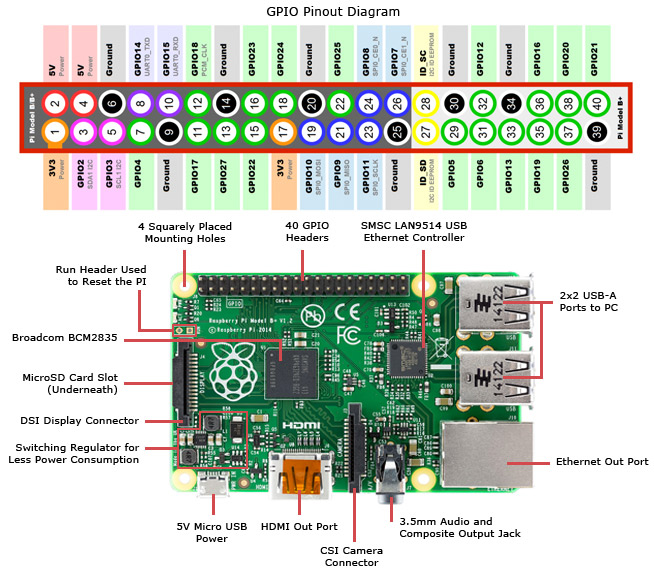
\includegraphics[scale=0.60]{figures/raspberry.jpg}
    \caption{اجزای رزبری‌پای مدل 3\lr{A}}
    \label{raspberry}
\end{figure}

\section{نمایشگر لمسی \lr{3.5} اینچی وِیوشِر}
<<<<<<< HEAD
این نمایشگر لمسی ساخت شرکت وِیوشِر\LTRfootnote{\lr{Waveshare}} بوده و دارای رزولوشن  {\lr{320x480} است. این نمایشگر را می‌توان برای انواع بوردهای رزبری‌پای مورد استفاده قرار داد. درایورهای این نمایشگر به صورت آماده بوده و به صورت مستقیم با  سیستم‌عامل رزبین هماهنگ است. اندازه‌ی این نمایشگر کاملاً با انواع بردهای رزبری‌پای مطابقت دارد و به راحتی بر روی آن قرار می‌گیرد. بر روی این نمایشگر می‌توان فیلم‌ها و عکس‌هایی با قالب‌\LTRfootnote{\lr{Format}} های مختلف و با کیفیتی بالا نمایش داد. این نمایشگر از نرم‌افزار صفحه‌کلید نیز پشتیبانی می‌کند که در این حالت نیازی به صفحه‌کلید خارجی نیست. صفحه لمسی این نمایشگر از نوع مقاومتی است. این نمایشگر در تصویر \ref{lcd} نشان داده شده است.
=======
این نمایشگر لمسی ساخت شرکت وِیوشِر\LTRfootnote{\lr{Waveshare}} بوده و دارای رزولوشن  {\lr{320x480} می باشد . این نمایشگر را می‌توان برای انواع بوردهای رزبری‌پای مورد استفاده قرار داد. درایورهای این نمایشگر به صورت آماده بوده و به صورت مستقیم با  سیستم‌عامل رزبین هماهنگ می‌باشد. اندازه‌ی این نمایشگر کاملاً با انواع بردهای رزبری‌پای مطابقت دارد و به راحتی بر روی آن قرار می‌گیرد. بر روی این نمایشگر می‌توان فیلم‌ها و عکس‌هایی با قالب‌\LTRfootnote{\lr{Format}} های مختلف و با کیفیتی بالا نمایش داد. این نمایشگر از نرم‌افزار صفحه‌کلید نیز پشتیبانی می‌کند که در این حالت نیازی به صفحه‌کلید خارجی نمی‌باشد. صفحه لمسی این نمایشگر از نوع مقاومتی می‌باشد. این نمایشگر در تصویر \ref{lcd} نشان داده شده است.
>>>>>>> 0b914906bc0a1f3ca7b01ffa78967759bf4780dc

\begin{figure}[t!]
    \centering
    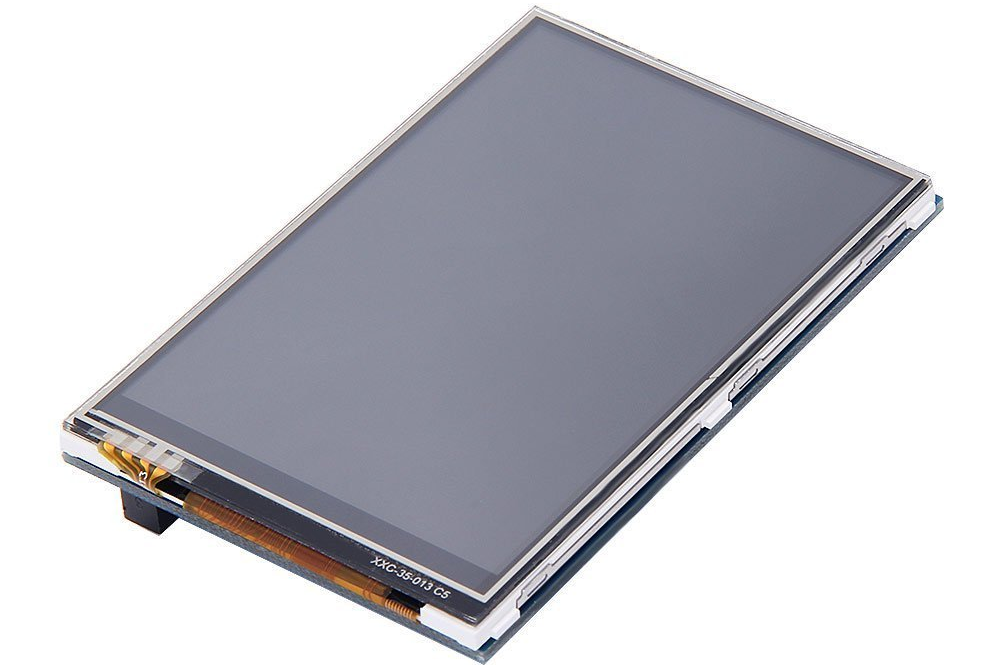
\includegraphics[scale=0.30]{figures/lcd.png}
    \caption{نمایشگر لمسی 3.5 اینچی}
    \label{lcd}
\end{figure}
\clearpage
برخی دیگر از ویژگی‌های این نمایشگر:

\begin{itemize}
	\item  یک جایگزین مناسب برای مانیتورهایی با رابط چندرسانه‌ای وضوح بالا
	\item پشتیبانی به‌وسیله درایورهای مورد نیاز
	\item پشتیبانی از سیستم‌عامل رزبین
	\item پشتیبانی از تمام نسخه‌های رزبری‌پای
	\item عکس‌برداری لمسی (در ۱۷ حالت دوربین)
	\item کیفیت بالای ساخت با روکش طلایی
	\item نمایشگر از جنس ترانزیستور فیلم نازک \LTRfootnote{\lr{TFT LCD}}
	\item رابط محیطی سریال \LTRfootnote{\lr{Serial Peripheral Interface (SPI)}}
	\item درایور لمسی \lr{XPT2046}
	\item پشتیبانی از ۶۵۵۳۶ رنگ مختلف
	\item نور پس‌زمینه از نوع دیود‌های ساطع‌کننده نور \LTRfootnote{\lr{Light-Emitting Diode (LED)}}
\end{itemize}


\section{سیستم‌عامل رزبین}
سیستم‌عامل نصب شده بر روی بورد رزبری‌پای، رزبین نام دارد. رزبین یک سیستم‌عامل رایانه‌ای مبتنی بر دبین\LTRfootnote{\lr{Debian}} برای رزبری‌پای است. نسخه‌های مختلفی از رزبین شامل \lr{Raspbian Buster} و \lr{Raspbian Stretch} وجود دارد.
این سیستم‌عامل را بنیاد رزبری از سال 2015 به طور رسمی به‌عنوان سیستم‌عامل اصلی برای خانواده رایانه‌های رزبری‌پای ارائه داده است. رزبین توسط مایک تامپسون\LTRfootnote{\lr{Mike Thompson}} و پیتر گرین\LTRfootnote{\lr{Peter Green}} به عنوان یک پروژه مستقل ایجاد شد. نسخه اولیه این سیستم‌عامل در ژوئن 2012 به پایان رسید. این سیستم‌عامل هنوز در حال توسعه است. رزبین برای پردازنده های آرم با توان پردازشی کم، بهینه شده است. رزبین در آخرین نسخه ارائه شده، از پیکسل\LTRfootnote{\lr{Pi Improved X-Window Environment, Lightweight(PIXEL)}} به عنوان محیط رومیزی\LTRfootnote{\lr{Desktop Enviorment}} خود استفاده می‌کند.

\section{چهارچوب نرم‌افزاری جنگو}
<<<<<<< HEAD
یک چهارچوب نرم‌افزاری\LTRfootnote{\lr{Software Framework}} سطح بالا، بسیاری از موارد برنامه نویسی را بصورت خودکار فراهم کرده و در اختیار برنامه نویس قرار می‌دهد . همچنین روش‌هایی میانبر و واسط برای اجرای اعمال مختلف را دارا است. این ویژگی باعث می‌شود برنامه‌نویس برای پیاده‌سازی بخش‌های مختلف کمتر کد بزند.
=======
یک چهارچوب نرم‌افزاری\LTRfootnote{\lr{Software Framework}} سطح بالا، بسیاری از موارد برنامه نویسی را بصورت خودکار فراهم کرده و در اختیار برنامه نویس قرار می‌دهد . همچنین روش‌هایی میانبر و واسط برای اجرای اعمال مختلف را دارا می‌باشد. این ویژگی باعث می‌شود برنامه‌نویس برای پیاده‌سازی بخش‌های مختلف کمتر کد بزند.
>>>>>>> 0b914906bc0a1f3ca7b01ffa78967759bf4780dc
جنگو\cite{Django}\LTRfootnote{\lr{Django}}  یک چارچوب نرم‌افزاری آزاد و متن‌باز\LTRfootnote{\lr{Open Source}} مبتنی بر پایتون\LTRfootnote{\lr{Python}} است که امکان طراحی و ایجاد بسیار سریع و آسان برنامه‌های تحت وب را فراهم می‌کند. جنگو از الگوی معماری \lr{MTV}\LTRfootnote{\lr{Model Template View}} پیروی می‌کند. این مؤسسه توسط بنیاد نرم افزاری مستقل جنگو\LTRfootnote{\lr{Django Software Independent Foundation}} تأسیس شده و نگهداری می‌شود.
هدف اصلی جنگو، سهولت در ایجاد وب‌سایت‌های پیچیده و با محوریت پایگاه‌داده است. این چارچوب بر ویژگی‌هایی از جمله استفاده مجدد\LTRfootnote{\lr{Reusability}} و تعداد خط کد کم\LTRfootnote{\lr{Less Code}}، وابستگی کم\LTRfootnote{\lr{Low Coupling}}، توسعه سریع\LTRfootnote{\lr{Rapid Development}} و اصل تکرار خود\LTRfootnote{\lr{Don't repeat yourself (DRY)}} تأکید دارد.
در این پروژه برای پیاده‌سازی ساختار کلی \lr{Back-end} و همچنین رابط کاربری مدیریت از جنگو استفاده شده است.

\subsection{مزیت‌های جنگو}
در ادامه ویژگی‌های این چهارچوب قدرتمند توضیح داده خواهد شد.
\subsubsection{امکان جداسازی محتوا از ظاهر نمایشی}
در اکثر زبان‌های برنامه‌نویسی، کدهای زبان نشانه‌گذاری ابرمتنی با کدها و محتوای سایت آمیخته می‌گردند، که باعث ایجاد مشکلات هنگام تغییرات آتی و نگهداری می‌گردد . با استفاده از این روش ظاهر نمایشی سایت، بصورت جداگانه در فایلی خاص ذخیره می‌گردد . اکنون با اعمال تغییر در هر نوع محتوا، نیازی به ویرایش دیگری نیست و این دو موجودیت مستقل می‌باشند.

\subsubsection{لایه‌بندی}
<<<<<<< HEAD
در حالت معمول هر برنامه نوشته شده با جنگو دارای ۳ لایه مهم است. بخش نمایشی\LTRfootnote{\lr{Template}}، محتوا و یا کدهای کنترلی\LTRfootnote{\lr{View}} و بخش ذخیره دائمی اطلاعات\LTRfootnote{\lr{Model}}. البته با توجه به نوع برنامه و نیاز‌های برنامه‌نویس می‌توان این لایه‌ها را ادغام کرده یا نادیده گرفت. نحوه ارتباط این لایه‌ها در تصویر\ref{mtv} نشان داده شده است.
=======
در حالت معمول هر برنامه نوشته شده با جنگو دارای ۳ لایه مهم می باشد. بخش نمایشی\LTRfootnote{\lr{Template}}، محتوا و یا کدهای کنترلی\LTRfootnote{\lr{View}} و بخش ذخیره دائمی اطلاعات\LTRfootnote{\lr{Model}}. البته با توجه به نوع برنامه و نیاز‌های برنامه‌نویس می‌توان این لایه‌ها را ادغام کرده یا نادیده گرفت. نحوه ارتباط این لایه‌ها در تصویر\ref{mtv} نشان داده شده است.
>>>>>>> 0b914906bc0a1f3ca7b01ffa78967759bf4780dc
 
\begin{figure}[t!]
    \centering
    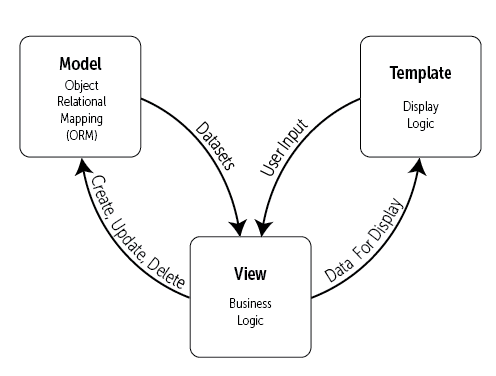
\includegraphics[scale=0.75]{figures/mtv.png}
    \caption{نحوه ارتباط لایه‌های جنگو}
    \label{mtv}
\end{figure}


\subsubsection{امکان استفاده موثر از سطح بالایی از تجرید و انتزاع}
جنگو در بسیاری از موارد با استفاده از مفهوم انتزاع، سهولت زیادی را فراهم کرده است. برای مثال برای کار با تکنولوژی‌هایی چون پروتکل انتقال پرونده\LTRfootnote{\lr{File Transfer Protocol;{FTP}}} یا زبان نشانه‌گذاری ابرمتنی\LTRfootnote{\lr{HyperText Markup Language}}، با یک مفهوم انتزاعی و سطح بالا روبرو خواهیم بود که با استفاده از روابط و توابع متعدد، برنامه‌نویسی را بسیار آسان و قدرتمند می‌کند.
 
علاوه بر موارد ذکر شده، جنگو ویژگی‌های دیگری نیز دارد. از جمله:
\begin{itemize}
	\item امکان تعیین اینکه کدام کد یا توابع مسئول جواب دادن به آدرس درخواست داده شده هستند.
<<<<<<< HEAD
	\item تسهیل نمایش، اعتبارسنجی و نمایش فرم‌های ساخته شده از زبان نشانه‌گذاری ابرمتنی یکی از مهترین روش‌ها برای دریافت اطلاعات از یک کاربر وب است.
=======
	\item تسهیل نمایش، اعتبارسنجی و نمایش فرم‌های ساخته شده از زبان نشانه‌گذاری ابرمتنی یکی از مهترین روش‌ها برای دریافت اطلاعات از یک کاربر وب می‌باشد.
>>>>>>> 0b914906bc0a1f3ca7b01ffa78967759bf4780dc
	\item حذف پسوند فایل از آدرس‌‌های وب (مثلا \lr{aspx.} یا \lr{php.})
\end{itemize}
 
\subsection{تاثیر پایتون بر روی جنگو}
همانطور که اشاره شد، جنگو بر اساس زبان برنامه‌نویسی پایتون نوشته شده که باعث شده است تا ویژگی‌های زبان پایتون برای جنگو نیز به ارث رسیده باشد. در زیر به برخی از این ویژگی‌ها اشاره شده است:
\begin{itemize}
	\item پایتون زبانی تفسیری\LTRfootnote{\lr{interpretive}} بوده و برای اجرا نیازی به کامپایل ندارد. این ویژگی باعث می‌شود که بعد از تغییر کد، نتایج کار بلافاصله قابل مشاهده باشد.
	\item داده‌ها و متغیر‌ها در پایتون پویا و بدون نیاز به تعریف نوع\LTRfootnote{\lr{Type}} هستند.
	\item نحو زبان پایتون کوتاه و در عین حال واضح و قابل فهم است. این ویژگی باعث می‌شود که برای انجام کارهای مشابه در زبان‌های برنامه‌نویسی دیگر، به نسبت کدنویسی کمتری انجام شود.
\end{itemize}

 
\subsection{بخش‌های جنگو}
در هسته جنگو، برای راحتی و سهولت کار بخش‌هایی طراحی و پیاده‌سازی شده است. برخی از 
این بخش‌ها عبارتند از:
\begin{itemize}
	\item میزبان وب مستقل و کوچک برای آزمون\LTRfootnote{\lr{Test}} برنامه 
	\item سیستمی برای معتبرسازی\LTRfootnote{\lr{Validation}} و سری‌سازی\LTRfootnote{\lr{Serialization}} فرم‌هایی با  زبان نشانه‌گذاری ابرمتنی
	\item چهارچوبی برای نهان‌سازی اطلاعات جهت استفاده مجدد با استفاده از حافظه نهان\LTRfootnote{\lr{Cache}} که روش‌های مختلف ذخیره و بازیابی حافظه نهان را در اختیار قرار می‌دهد .
	\item پشتیبانی از ابزارهای میانی\LTRfootnote{\lr{Middleware}} که امکان اجرای توابع و دستورات مورد نظر را در مراحل مختلف پردازش یک درخواست ،فراهم می‌کند.
	\item یک توزیع‌کننده\LTRfootnote{\lr{Dispatcher}} درونی که به بخش‌های مختلف برنامه امکان دریافت سیگنال‌ها و رویدادهای مختلف را می‌دهد.
	\item سیستم بین‌الملل‌سازی\LTRfootnote{\lr{Internationalization}} که حتی امکان ترجمه بخش‌های مختلف جنگو به زبان‌های مختلف را فراهم می‌کند. از این ویژگی جهت تنظیم ساعت محلی نیز استفاده می‌شود.
<<<<<<< HEAD
	\item  سیستمی برای تسلسل و سری‌سازی که امکان کار با انواع داده‌های مبتنی بر زبان نشانه گذاری امتدادپذیر\LTRfootnote{\lr{eXtensible Markup Language (XML)}} و نماد شئ جاوااسکریپت\LTRfootnote{\lr{JavaScript Object Notation (JSON)}} را فراهم می کند .
	\item سیستمی برای توسعه قابلیت‌های موتور قالب. مانند تعیین دسترسی برای هر بخش مختلف از سایت.
\end{itemize}
 
همچنین بسته جنگو شامل ابزارها و برنامه‌های جانبی مختلفی است که در داخل بسته \lr{contrib} قرار دارند. برخی از این ابزار ها عبارتند از:
=======
	\item  سیستمی برای تسلسل و سری‌سازی که امکان کار با انواع داده‌های مبتنی بر زبان نشانه گذاری امتدادپذیر\LTRfootnote{\lr{eXtensible Markup Language (XML)}} و نماد شئ جاوااسکریپ\LTRfootnote{\lr{JavaScript Object Notation (JSON)}} را فراهم می کند .
	\item سیستمی برای توسعه قابلیت‌های موتور قالب. مانند تعیین دسترسی برای هر بخش مختلف از سایت.
\end{itemize}
 
همچنین بسته جنگو شامل ابزارها و برنامه‌های جانبی مختلفی می‌باشد که در داخل بسته \lr{contrib} قرار دارند. برخی از این ابزار ها عبارتند از:
>>>>>>> 0b914906bc0a1f3ca7b01ffa78967759bf4780dc
\begin{itemize}
	\item سیستم تصدیق و شناسایی کاربر\LTRfootnote{\lr{Authentication}}
	\item سیستم تعیین دسترسی به کاربر\LTRfootnote{\lr{Authorization}}
	\item رابط مدیریتی پویا
	\item ابزارهایی برای ایجاد \lr{RSS} و \lr{Atom}
	\item سیستم نظر‌دهی انعطاف‌پذیر
	\item یک چارچوب برای ایجاد برنامه‌های کاربردی \lr{GIS}
	\item ابزارهایی برای تولید نقشه سایت\LTRfootnote{\lr{Sitemap}}
	\item ابزارهای امنیتی برای جلوگیری از حملات \lr{CSRF}
	\item کتابخانه‌های قالب که امکان استفاده از زبان‌های نشانه‌گذاری کم حجم مانند \lr{Textile} و \lr{Markdown} را فراهم می‌سازد.
\end{itemize}
 
\subsection{انطباق با میزبان‌های مختلف}
<<<<<<< HEAD
جنگو با استفاده از واحد\LTRfootnote{\lr{Module}} \lr{mod\_python} به‌خوبی بر روی میزبان‌های وب آپاچی\LTRfootnote{\lr{Apache}} قابل اجرا است. همچنین بر روی تمامی میزبان‌هایی که از \lr{WSGI}پشتیبانی می‌کنند قابل اجرا است. به غیر از موارد ذکر شده، جنگو توانایی راه‌اندازی سرور \lr{FastCGI} را دارا است.
=======
جنگو با استفاده از واحد\LTRfootnote{\lr{Module}} \lr{mod\_python} به‌خوبی بر روی میزبان‌های وب آپاچی\LTRfootnote{\lr{Apache}} قابل اجرا است. همچنین بر روی تمامی میزبان‌هایی که از \lr{WSGI}پشتیبانی می‌کنند قابل اجرا می‌باشد. به غیر از موارد ذکر شده، جنگو توانایی راه‌اندازی سرور \lr{FastCGI} را دارا می‌باشد.
>>>>>>> 0b914906bc0a1f3ca7b01ffa78967759bf4780dc
 
\section{چهارچوب نرم‌افزاری \lr{REST} جنگو}
برای آشنایی با این چهارچوب، ابتدا دو موضوع رابط‌برنامه‌نویسی نرم‌افزار\LTRfootnote{\lr{Application Programming Interface (API)}} و \lr{REST} باید توضیح داده شود.
 
\subsection{رابط برنامه‌نویسی نرم‌افزار چیست؟}
در حوزه توسعه نرم‌افزار، واژه‌ رابط برنامه‌نویسی نرم‌افزار بسیار تکرار می‌شود. در واقع، از آنجا که می‌توان واژه \lr{Interface} را به «فصل مشترک» در فارسی ترجمه کرد، می‌توان گفت که رابط برنامه‌نویسی نرم‌افزار فصل مشترکی مابین دو نرم‌افزار یا اپلیکیشن است.
\subsubsection{آشنایی با انواع رابط‌های برنامه‌نویسی نرم‌افزار}
با در نظر گرفتن این نکته که رابط‌ برنامه‌نویسی نرم‌افزار سازوکاری است که از طریق آن تعامل سیستم با سیستم به جای تعامل کاربر با سیستم صورت می‌گیرد، می‌توان دسته‌بند‌ی‌های مختلفی در نظر گرفت که عبارتند از:

\begin{itemize}
	\item رابط برنامه‌نویسی در سخت‌افزار
	\item رابط برنامه‌نویسی نرم‌افزاری در سطح سیستم‌عامل
	\item رابط برنامه‌نویسی نرم‌افزاری در زبان‌های برنامه‌نویسی
	\item کیت‌های توسعه نرم‌افزار\LTRfootnote{\lr{Software Development Kit (SDK)}}
	\item رابط برنامه‌نویسی نرم‌افزاری تحت وب (وب سرویس)
\end{itemize}
 

\subsubsection{تقسیم‌بندی رابط‌های برنامه‌نویسی نرم‌افزار از بُعد سطح دسترسی}
علاوه بر تقسیم‌بندی‌های فوق،‌ رابط برنامه‌نویسی نرم‌افزارهای تحت وب را می‌توان از نقطه نظر سطح دسترسی به دسته‌های مختلفی تقسیم‌بندی کرد که عبارتند از:
\begin{itemize}
	\item رابط برنامه‌نویسی نرم‌افزار باز\LTRfootnote{\lr{Open API}}: این دست رابط‌های برنامه‌نویسی نرم‌افزار که اصطلاحاً \lr{Public APIs} نیز نامیده می‌شوند، بدون هیچ‌گونه محدودیت در سطح دسترسی برای کاربردهای مجموعه‌های تجاری به مشتری\LTRfootnote{\lr{Business to Customer (B2C)}}، در اختیار برنامه‌نویس‌ها قرار می‌گیرند.
	\item رابط برنامه‌نویسی نرم‌افزار شریک\LTRfootnote{\lr{Partner API}}: این گروه از رابط‌های برنامه‌نویسی نرم‌افزار صرفاً در اختیار کسب‌وکارهای به اصطلاح تجاری به تجاری\LTRfootnote{\lr{Business to Business (B2B)}} و تجاری به مشتری است و برخلاف مورد قبل هر برنامه‌نویسی به آن‌ها دسترسی ندارد؛ برای استفاده از آن‌ها معمولا باید هزینه کرد.
	\item رابط برنامه‌نویسی نرم‌افزار داخلی \LTRfootnote{\lr{Internal API}}: این گروه از رابط‌های برنامه‌نویسی نرم‌افزار که تحت عنوان \lr{Private APIs} نیز شناخته می‌شوند، صرفاً برای استفاده‌های داخلی یک سیستم طراحی می‌شوند.

\end{itemize}

\subsection{\lr{REST} چیست؟}
<<<<<<< HEAD
با توجه به تعریف
=======
با توجه به تعریف \cite{REST}
>>>>>>> 0b914906bc0a1f3ca7b01ffa78967759bf4780dc
\lr{REST}\LTRfootnote{\lr{Representational State Transfer}} يك مدل معماري براي طراحي برنامه‌هاي كاربردی شبكه است. ايده اصلي این معماری اين است كه به جاي استفاده از مكانيزم‌هاي پيچيده‌اي مانند \lr{CORBA}، \lr{RPC} يا \lr{SOAP} براي اتصال ماشين‌ها، از \lr{HTTP} و به سادگی براي برقراري ارتباط بين ماشين‌ها استفاده شود.\\
این مدل دارای ویژگی‌های زیر است: 
\begin{itemize}
	\item بر پایه مشتری-میزبان\LTRfootnote{\lr{client-server}} است.
	\item بدون حالت\LTRfootnote{\lr{Stateless}} است.
	\item از حافظه نهان\LTRfootnote{\lr{Cache}} پشتیبانی می‌کند.
	\item سيستم لايه‌بندي شده است.
    \item دارای واسط واحد\LTRfootnote{\lr{Uniform Interface}} است.
\end{itemize}
 
به سيستمي كه اين قيود را رعايت نمايد، \lr{RESTful} مي‌گويند. از لحاظ رويكرد برنامه‌نويسي \lr{REST} جايگزيني ساده براي سرويس‌هاي وب است. توسعه‌پذيري در تعاملات ميان اجزا، عموميت واسط‌ها و توسعه مستقل اجزا از كليدي‌ترين اهداف این معماری است.

استفاده از معماري \lr{REST} در برنامه‌نويسي، كارايي، سادگي، انعطاف‌پذيري، امكان مشاهده و نظارت، قابليت حمل و قابليت اطمينان را افزايش مي دهد.
امروزه برنامه‌های سنتی وب در حال حرکت به سمت سرویسی شدن هستند. بدین صورت که برنامه سمت مشتری تنها از طریق وب‌سرویس‌ها با سرور در تماس هستند. به بیانی دیگر ارتباط سمت مشتری با لایه داده برنامه، از طریق وب‌سرویس‌ها صورت می‌پذیرد. در چنین برنامه‌هایی منطق برنامه کاملا در سمت مشتری پیاده‌سازی می‌شود و سمت میزبان دیگر هیچ نقشی جز فراهم‌کردن داده برای برنامه‌های سمت مشتری را برعهده ندارد.
 
یکی از نکات مثبت این معماری این است که دسترسی برنامه سمت مشتری به منابع، از طریق درخواست‌های \lr{HTTP} انجام می‌گیرد. این درخواست‌ها با روش\LTRfootnote{\lr{Method}}های مختلفی می‌توانند ارسال شوند که هر یک معنا و مفهومی خاصی دارد. هریک از این روش‌ها در زیر تعریف شده‌اند:
\begin{itemize}
	\item روش \lr{GET} به‌منظور بازیابی و خواندن منبع استفاده می شود.
	\item روش \lr{POST} زمانی استفاده می‌شود که بخواهیم منبع جدیدی را ایجاد کنیم.
	\item روش \lr{DELETE} به‌منظور حذف یک منبع مورد استفاده قرار می‌گیرد.
	\item روش‌های \lr{PUT} و \lr{PATCH} برای دست‌کاری در یک منبع مورد استفاده قرار می‌گیرند.
\end{itemize}


\subsection{جنگو \lr{REST}}
چهارچوب نرم‌افزاری جنگو \lr{REST}\cite{DjangoREST}، یک ابزار قدرتمند و انعطاف‌پذیر برای ساختن رابط‌های برنامه‌نویسی نرم‌افزارهای شبکه وب است.
برخی از ویژگی‌های این چهارچوب نرم‌افزاری به صورت زیر است:
\begin{itemize}
	\item خط مشی‌های تأیید اعتبار شامل بسته‌هایی برای \lr{OAuth1a} و \lr{OAuth2}
	\item پشتیبانی از منابع داده \lr{ORM}\LTRfootnote{\lr{Object-Relational Mapping}} و غیر \lr{ORM}
	\item مستندات گسترده و پشتیبانی 
	\item مورد استفاده و مورد اعتماد شرکت‌های معتبر بین المللی از جمله موزیلا، \lr{Red Hat}، \lr{Heroku} و \lr{Eventbrite} است.
\end{itemize}


\section{چهارچوب نرم‌افزاری \lr{Vue.js}}
\lr{Vue.js}\cite{Vue} یک چارچوب متن باز \lr{JavaScript} برای ساخت رابط‌های کاربری\LTRfootnote{\lr{User Interface}} و برنامه‌های تک‌صفحه‌ای\LTRfootnote{\lr{Single Page Application}} است. این چهارچوب نخستین بار توسط ایوان یو\LTRfootnote{\lr{Evan You}} ایجاد شده است و اکنون توسط او و بقیه اعضای تیم اصلی که از شرکت‌های مختلفی چون \lr{Netlify} و \lr{Netguru} آمده‌اند، نگهداری می‌شود.

در ادامه برخی از ویژگی‌های این چهارچوب توضیح داده خواهد شد.

\subsection{اجزاء}
هدف این اجزا\LTRfootnote{\lr{Componenets}}، افزایش استفاده مجدد از کد است. در مواقعی که در چندین بخش مختلف به یک المان خاص در طراحی صفحات نیاز است، از این اجزا استفاده می‌شود.

\subsection{قالب‌ها}
\lr{Vue} از یک نحو\LTRfootnote{\lr{Syntax}} که مشابه قوانین نوشتاری زبان نشانه‌گذاری ابرمتنی است، استفاده می‌کند. همه قالب‌های \lr{Vue} دارای زبان نشانه‌گذاری ابرمتنی معتبری هستند که توسط مرورگرهای استاندارد قابل تجزیه\LTRfootnote{\lr{Parse}} است. \lr{Vue} این امکان را می‌دهد تا قالب‌ها قبل از بروزرسانی مرورگر، تغییرات لازم را اعمال کنند.

کاربران \lr{Vue} می توانند از نحو استاندارد در قالب‌ها استفاده کنند و مستقیماً و با استفاده از \lr{JSX} بنویسند.


\subsection{انتقال‌ها}
{\lr{Vue}} روش‌های مختلفی را برای اعمال جلوه‌های انتقال \LTRfootnote{\lr{Transitions}}هنگام وارد کردن، به روزرسانی یا حذف شدن از \LTRfootnote{\lr{Document Object Model}}\lr{DOM} را فراهم کرده است. این موارد عبارتند از:

\begin{itemize}
   	\item اعمال خودکار کلاس‌ها برای انتقال‌ها و انیمیشن‌های \lr{CSS}
   	\item تعامل با کتابخانه‌های شخص ثالث \lr{CSS}، مانند \lr{Animate.css}
   	\item تعامل با کتابخانه‌های شخص ثالث جاوا اسکریپت ، مانند \lr{Velocity.js}
\end{itemize}




\subsection{چهارچوب نرم‌افزاری \lr{Nuxt.js}}
\lr{Nuxt.js}\cite{Nuxt} یک چارچوب برنامه وبِ منبع آزاد و مبتنی بر \lr{Vue.js} ، \lr{Node.js} ، \lr{Webpack} و \lr{Babel.js} است.
  ابتدا به معرفی \lr{Vue.js} پرداخته می‌شود.

از مزایای استفاده از این چهارچوب\LTRfootnote{\lr{Framework}}، کاهش زمان پاسخگویی برنامه و همچنین بهبود بهینه سازی موتور جستجو\LTRfootnote{\lr{SEO}} در مقایسه با سایر برنامه‌های تک‌صفحه‌ای است. دلیل کاهش زمان تعامل این است که محتوای کامل هر صفحه، قبل از اجرای جاوا اسکریپت در برنامه سمت مشتری، توسط وب سرور ارائه\LTRfootnote{\lr{Render}} می‌شود. به بیان دیگر، با استفاده از این چهارچوب، به‌طور همزمان از مزایای نمایش سنتی \lr{HTML} و همچنین نمایش به وسیله برنامه‌های تک‌صفحه‌ای جدید بهره برده می‌شود.
اما فایده اصلی این چهارچوب، ساده‌سازی و یکپارچه‌سازی پروژه سمت کاربر برای برنامه‌نویس است.


\section{پایگاه‌داده رابطه‌ای \lr{Postgress}}
<<<<<<< HEAD
\lr{Postgress}\cite{Postgress}، که همچنین با عنوان \lr{Postgres} شناخته می‌شود، یک سیستم مدیریت پایگاه‌داده رابطه‌ای\LTRfootnote{\lr{Relational}} آزاد و متن‌باز است. ابتدا به مفاهیم پایگاه‌داده رابطه‌ای پرداخته می‌شود و سپس پایگاه‌داده \lr{Postgress} معرفی می‌گردد.
=======
\lr{Postgress}\cite{Postgress}، که همچنین با عنوان \lr{Postgres} شناخته می‌شود، یک سیستم مدیریت پایگاه‌داده رابطه‌ای\LTRfootnote{\lr{Relational}} آزاد و متن‌بازاست. ابتدا به مفاهیم پایگاه‌داده رابطه‌ای پرداخته می‌شود و سپس پایگاه‌داده \lr{Postgress} معرفی می‌گردد.
>>>>>>> 0b914906bc0a1f3ca7b01ffa78967759bf4780dc
 
\subsection{پایگاه داده رابطه‌ای}
پایگاه داده رابطه‌ای به آن دسته از پایگاه‌های داده اطلاق می‌شود که بر اساس مدل رابطه‌ای طراحی و ایجاد شده باشند. پس از پایگاه‌های داده‌ای سلسله مراتبی و شبکه‌ای، که هر یک دارای ضعف‌هایی بودند، متخصصان در جستجوی مدلی بودند که دارای ساختار داده‌ای با انتزاع قوی باشد. مدل رابطه‌ای در سال ۱۹۷۰ توسط ادگار کاد\LTRfootnote{\lr{Edgar F.Codd}} مطرح شد. این مدل دارای ساختار داده‌ای با انتزاع قوی بوده و اساساً ساختار داده‌ای در آن بر اساس یک مفهوم ریاضی به نام رابطه استوار است. در اینجا لازم است به این نکته توجه شود که مفهوم رابطه با مفهوم ریاضی آن تاحدودی متفاوت است.
 
برای طراحی پایگاه داده‌ها در سطح انتزاعی پایین‌تر از سطح مدل‌سازی، به یک ساختار داده‌ای از یک مدل داده‌ای نیاز است و اساساً همین مدل داده‌ای تأمین‌کننده محیط انتزاعی است. در پایگاه داده رابطه‌ای بالاخص در محیط انتزاعی مورد استفاده کاربر، رابطه نمایشی جدولی دارد و اساساً پایگاه داده رابطه‌ای مجموعه‌ای است از تعدادی نوع جدول. مفاهیم ساختار جدولی عبارتند از: سطر، جدول و ستون
هر جدول از نظر محتوای داده‌ای مجموعه‌ای است از نمونه‌های متمایز از انواع سطرها و هر سطر نیز مجموعه‌ای از مقادیر است که هر کدام از یک مجموعه برگرفته شده‌اند. به هر یک از عناصر سطر یک ستون گویند. لازم است ذکر شود که در ساختار جدولی، تنها عنصر ساختاری اساسی همین مفهوم نوع جدول است.
 
\subsubsection{ویژگی‌های رابطه}
<<<<<<< HEAD
رابطه به عنوان تنها عنصر ساختاری اصلی در مدل رابطه‌ای برای نمایش انواع موجودیت‌ها و انواع ارتباطات به کار می‌رود. در واقع در مدل رابطه‌ای هم نوع موجودیت و هم نوع ارتباط با مفهوم رابطه نمایش داده می‌شوند و در نتیجه هم نمونه موجودیت و هم نمونه ارتباط با مفهوم تاپل نشان داده می‌شوند. رابطه دارای چهار ویژگی زیر است:
=======
رابطه به عنوان تنها عنصر ساختاری اصلی در مدل رابطه‌ای برای نمایش انواع موجودیت‌ها و انواع ارتباطات به کار می‌رود. در واقع در مدل رابطه‌ای هم نوع موجودیت و هم نوع ارتباط با مفهوم رابطه نمایش داده می‌شوند و در نتیجه هم نمونه موجودیت و هم نمونه ارتباط با مفهوم تاپل نشان داده می‌شوند. رابطه دارای چهار ویژگی زیر می‌باشد:
>>>>>>> 0b914906bc0a1f3ca7b01ffa78967759bf4780dc
\begin{itemize}
  	\item رابطه تاپل تکراری ندارد، زیرا بدنه رابطه مجموعه‌است و مجموعه نمی‌تواند عنصر تکراری داشته باشد.
	\item تاپل‌ها نظم ندارند زیرا بدنه رابطه مجموعه‌ است و مجموعه در حالت کلی فاقد نظم است.
	\item صفات رابطه نظم مکانی ندارند زیرا سرآیند، رابطه مجموعه‌است و مجموعه در حالت کلی فاقد نظم است.
	\item تمام صفات تک مقداری (تجزیه نشدنی) هستند زیرا در نمایش جدولی رابطه، در تقاطع هر سطر و ستون باید یک مقدار وجود داشته باشد.
\end{itemize}

 
\subsubsection{انواع کلیدها در مدل رابطه‌ای}

\begin{itemize}
  	\item ابر کلید: هر ترکیبی از صفات جدول را که یکتایی مقدار داشته باشد، ابر کلید گویند. به بیانی دیگر هر زیر مجموعه عنوان رابطه را دارد، که یکتایی مقدار در بدنه رابطه را داشته باشد. تعریف دیگر ابر کلید عبارت است از هر ترکیبی از اسامی صفات رابطه که در هیچ دو تاپل مقدار یکسان نداشته باشد.

  	\item کلید کاندید: کلید کاندید امکانی است برای ارجاع به «تک تاپل» در رابطه. مجموعه صفات \lr{k} از رابطه\lr{R} یک کلید کاندید است، اگر دارای خاصیت غیر کاهشی و یکتایی باشد.

  	\item کلید اصلی: 
  	\item یکی از کلیدهای کاندید رابطه که شرایط زیر را داشته باشد:
	\begin{enumerate}
		\item شناسایی‌کننده نوع موجودیت در رابطه باشد. مانند شماره عضویت کتابخانه برای هر دانشجو.
		\item از نظر طول، کوتاه‌تر باشد. یعنی بین دو کلید کاندید، کلید کوتاه‌تر برای کلید اصلی بودن بهتر است.
	\end{enumerate}
  	\item کلید جانشین: هر کلید کاندید به غیر از کلید اصلی را کلید جانشین گویند.
  	\item کلید خارجی: دو رابطه \lr{R1} و \lr{R2} را در نظر بگیرید. هر زیر مجموعه از صفات رابطه \lr{R2}که هر مقدار معلوم آن با یک مقدار از کلید کاندید \lr{R1}برابر باشد، کلید خارجی در رابطه \lr{R2}است. نقش کلید خارجی برای نمایش ارتباطات بین انواع موجودیت‌ها و در نتیجه بین نمونه‌های آنها به کار می‌رود.

\end{itemize}


 
\subsection{پایگاه‌داده \lr{Postgress}}
\lr{Postgress} یک سامانه مدیریت پایگاه داده‌های رابطه‌ای است که برای سیستم‌های مختلفی از جمله لینوکس، فری بی‌اس‌دی\LTRfootnote{\lr{FreeBSD }}، ویندوز و مک اواس\lr{macOS} موجود است. این پایگاه‌داده توسط گروه توسعه سراسری \lr{Postgresql} توسعه داده می‌شود، که شامل تعداد زیادی از افراد داوطلب است. این پایگاه‌داده بر توسعه‌پذیری و رعایت استانداردهای فنی تأکید دارد. همچنین توانایی پاسخگویی به بار کاری زیاد، در مقیاس یک کامپیوتر تا انبارهای داده،\LTRfootnote{\lr{Data Warehouse}} برای استفاده همزمان کاربران را دارد.
 
تراکنش‌های \lr{PostgreSQL} شامل ویژگی‌های زیر است:
\begin{itemize}
  	\item اتمی\LTRfootnote{\lr{Atomicity}}
	\item پایداری\LTRfootnote{\lr{Consistency}}
	\item ایزوله\LTRfootnote{\lr{Isolation}}
	\item با دوام\LTRfootnote{\lr{Durability}}
	\item بروزرسانی خودکار نمایه‌ها\LTRfootnote{\lr{Automatically Updatable Views}}
	\item پشتیبانی از تریگر\LTRfootnote{\lr{Trigger}}
	\item پشتیبانی از کلید‌های خارجی
	\item پشتیبانی از توابع تجمیعی
	\item کلید‌های خارجی
	\item پشتیبانی از رویه‌های ذخیره‌شده\LTRfootnote{\lr{Stored Procedures}}
\end{itemize}


\section{ماشین مجازی}
برای پیاده‌سازی این پروژه در محیط عملیاتی از میزبان مجازی شخصی\LTRfootnote{\lr{Virtual Private Server (VPS)}} استفاده شده است. برای این که بدانیم میزبان مجازی شخصی چیست، ابتدا باید با ماشین مجازی\LTRfootnote{\lr{Virtual Machine}} آشنا شویم. یک ماشین مجازی از منابع فیزیکی یک کامپیوتر استفاده می کند. این منابع می توانند پردازنده، حافظه رم و یا دیسک‌های ذخیره‌سازی باشند. ماشین‌های مجازی با بهره‌گیری از این منابع، یک نوع از کامپیوتر را شبیه‌سازی می‌کنند.
برای درک بهتر، کافی است امکان تصویر در تصویر یک تلویزیون را تصور کنید. یک تلویزیون امروزی می‌تواند همزمان دو تصویر از دو شبکه متفاوت را پخش کند. این امکان در حالی برای شما فراهم می‌شود که در حال استفاده از یک تلویزیون هستید؛ اما نتیجه‌ای که حاصل می‌شود، دو تصویر همزمان است. پس در این حالت از یک منبع واحد، حداقل دو خروجی دریافت کرده‌اید. پس یک یا چند ماشین‌ مجازی می‌تواند درون یک سخت‌افزار یک کامپیوتر واحد اجرا شود. به‌عنوان مثال می‌توان یک ماشین‌ مجازی با سیستم‌عامل ویندوز را درون یک کامپیوتر که خود نیز از سیستم‌عامل ویندوز بهره می‌برد اجرا کرد.
این امکان وجود دارد که چندین سیستم‌عامل را از طریق ماشین‌های مجازی به واسطه یک سخت‌افزار واحد اجرا کرد. این دقیقا همان کاری است که شرکت های ارائه میزبانی\LTRfootnote{\lr{Hosting}} انجام می‌دهند. اما این بار تفاوت آن‌جا است که آن‌ها به جای کامپیوترهای شخصی از سرورهای پرقدرت استفاده می‌کنند. سرورهایی که هرکدامشان می‌توانند بیش از 48 هسته پردازشگر و بیش از 1 ترابایت حافظه رم داشته باشند. تعداد زیادی از این سرورها در محل‌هایی به نام مراکز داده\LTRfootnote{\lr{Data center}} نگه‌داری می شوند. هر مرکز داده نیز می‌تواند بیش از صدها و شاید هزاران سرور را درون خود جای دهد. هر کدام از این سرورها نیز توانایی اجرای چندین و شاید صدها ماشین مجازی را دارند.
این ماشین‌های مجازی می‌توانند توسط سازمان‌ها، ادارات و یا حتی افراد استفاده شوند. اگر یک ماشین مجازی اجاره داده شود، اصطلاحا به آن سرور اختصاصی مجازی یا میزبان مجازی شخصی می‌گویند. پس بنابراین یک میزبان مجازی شخصی یک ماشین مجازی به حساب می‌آید و فقط نام تجاری به خود گرفته‌است.
 
\subsection{دلایل استفاده از میزبان مجازی شخصی}
میزبان مجازی شخصی به عنوان یک سرویس به کاربر ارائه می‌شود. اما دیگر سرویس‌هایی که در مقابل میزبان مجازی شخصی قرار می‌گیرند، هاست‌های اختصاصی و هاست‌های اشتراکی هستند.
هاست‌های اختصاصی به صورت کامل در اختیار کاربران قرار می‌گیرند. به این صورت که مشتری یک سرور کامل را اجاره کرده و آن را در تحت نظارت و استفاده می‌گیرد. به این ترتیب هیچ‌کس دیگری به آن سخت‌افزار دسترسی نداشته و کنترل کامل سخت افزار در اختیار اجاره کننده‌است.
درمقابل، هاستینگ اشتراکی بدین معناست که در یک سرور واحد، چندین برنامه اجرا شده و چندین مشتری همزمان از سخت‌افزار استفاده می‌کنند.
هاست‌های اختصاصی معمولا از منابع سخت‌افزاری غنی‌تری نسبت به میزبان مجازی شخصی بهره برده و البته اجاره آن‌ها نیز بسیار گران است. درحالی که اجاره میزبان‌های اشتراکی نسبت به هاست‌های اختصاصی ارزان‌تر بوده ولی به هیچ عنوان انعطاف‌پذیری میزبان مجازی شخصی را ندارند.
می‌توان گفت اجاره یک میزبان مجازی شخصی نیز فقط کمی گران‌تر از هاست‌های اشتراکی است. 
میزبان مجازی شخصی قابل انعطاف است. چرا که شما تقریبا هرکاری را می‌توانید با یک ماشین مجازی ویندوزی انجام دهید. می توان از یک میزبان مجازی شخصی به‌عنوان فضایی برای ذخیره‌سازی اطلاعات شخصی استفاده کرد.

نکته ای راجع به یک میزبان مجازی شخصی باید در نظر گرفته شود، این است که درصورت استفاده نادرست از آن، کاربر نمی‌تواند هیچ‌گونه آسیبی به سرور اصلی بزند. به عنوان مثال اگر یک میزبان مجازی شخصی آلوده به ویروس شود، دیگر ماشین‌های مجازی موجود در سرور در امان خواهند بود و کوچک‌ترین اختلالی در نحوه سرویس‌دهی آن‌ها پیش نخواهد آمد.
یک میزبان مجازی شخصی می‌تواند به راحتی راه‌اندازی مجدد شده و یا حتی در عرض چند دقیقه دوباره با یک سیستم‌عامل جدید در اختیار کاربر قرار گیرد. تنها نکته‌ای که باید مدنظر داشت، تهیه نسخه پشتیبان از اطلاعات حیاتی است، چرا که آن ها هنگام نصبِ دوباره سیستم‌عامل از بین خواهند رفت.
ماشین‌های مجازی ایمن هستند. به این معنی که هر ماشین مجازی به صورت جداگانه از منابع استفاده کرده و دسترسی کاربران به ماشین مجازی فرد دیگری، غیرممکن است.
اما این مهم درصورت استفاده از میزبان‌های اشتراکی کمی متفاوت است. به دلیل قرارگیری اپلیکیشن‌ها و یا وب‌سایت ها در کنار همدیگر و مدیریت آن‌ها توسط نرم‌افزاری واحد مانند وب‌سرورها؛ امکان این که دیگر اپلیکیشن ها مورد سوءاستفاده توسط دیگر کاربران قرار گیرد، وجود دارد.
 

\subsection{موارد استفاده از میزبان مجازی شخصی}
در ذیل به مواردی خواهیم پرداخت که با استفاده از یک میزبان مجازی شخصی می توان به آن‌ها دست پیدا کرد.

\subsubsection{اجرای یک وب‌سایت}
این روزها بهترین راه اجرای یک وب‌سایت از طریق میزبان مجازی شخصی است. معمولا برای یک میزبان مجازی شخصی منابع اختصاصی در نظر گرفته می‌شود. به این‌صورت که بخشی از منابع که اختیار کرده اید، همواره در اختیار شما خواهد بود و برنامه دیگری امکان اشغال آن را ندارد.

\subsubsection{ایجاد یک سرور یا سرویس}
شاید یک سازمان، شرکت و یا حتی اشخاص بخواهند برای خود سرویس ایمیل اختصاصی داشته باشند. با استفاده از میزبان مجازی شخصی و نرم‌افزار سرویس ایمیل می‌توان سرور اختصاصی پست الکترونیک خود را داشته و شخصا آن را مدیریت کرد. این راه کار بسیار مورد استقبال شرکت‌ها قرار گرفته است.


\subsubsection{ایجاد یک محیط آزمایشی}
با استفاده از یک میزبان مجازی شخصی می‌توان به آزمایش و اصلاح انواع نرم افزارهای گوناگون پرداخت. اشاره شد که اگر اتفاق ناگواری برای یک میزبان مجازی شخصی بیافتد دیگر ماشین‌های مجازی از این رخداد صدمه‌ای نخواهند دید. درصورتی که سیستم‌عامل یک میزبان مجازی شخصی دچار اشکال شود، به راحتی هرچه تمام‌تر می توان سیستم‌عامل جدیدی را جایگزین کرد. این در صورتی است که اگر این اتفاق برای یک هاست اختصاصی رخ دهد، نصب و راه‌اندازی یک سیستم‌عامل جدید کاری پردردسر و زمان‌بر خواهد بود.


\section{نتیجه‌گیری}
همانطور که در قسمت‌های مختلف این بخش به تفصیل توضیح داده شد، این پروژه از قطعات سخت‌افزاری، تکنولوژی‌های نرم‌افزاری و همچنین محیط‌هایی برای عملیاتی کردن استفاده شده است. برای پیاده‌سازی سخت‌افزاری پروژه از بورد رزبری‌پای مدل \lr{3A} استفاده شد. همچنین جهت تعامل این بورد با کاربر، از نمایشگر لمسی \lr{3.5} اینچی \lr{Waveshare} استفاده شد. برنامه‌ای که بر روی نمایشگر نمایش داده می‌شود، با استفاده از چهارچوب نرم‌افزاری سمت کاربر \lr{Nuxt.js} که خود بر پایه \lr{Vue.js} نوشته شده است، برنامه‌نویسی شد. این برنامه با استفاده از وب‌سرویس \lr{REST} با چهارچوب نرم‌افزاری \lr{Django} در تعامل است.

برای عملیاتی کردن پروژه بر روی محیطی که همه کاربران به برنامه‌ها دسترسی داشته باشند از ماشین مجازی استفاده شد.




\chapter{مشخصات یک پایان نامه و گزارش علمی}

اگرچه براي همه انواع نوشته‌ها، مشخصات و ويژگي‌هاي واحد و معيني نمي‌توان ذكر كرد، با اين حال در یک پایان نامه یا گزارش علمی باید نکات و موارد کلی که در این فصل ذکر می‌شود، بطور کامل رعایت شده باشد. 

دقت كنيد كه پس از عنوان فصل بايد حداقل توضیحی کوتاه در مورد موضوع نوشته شود و نمي‌توان مستقيماً بعد از آن عنوان بخش را نوشت و همين طور پس از عناوين بخش‌ها و زيربخش‌ها.(مانند دستورالعمل حاضر)
\section{برخورداری از غنای علمی }

يك پایان نامه بايد پیش از هر چيز به‌لحاظ علمي از غناي لازم برخوردار باشد. يعني هدف و پيام روشني داشته باشد و از پيش‌زمينه علمي، بيان دلايل علمی، ارجاعات مورد نیاز و نتيجه‌گيري شفاف بهره ببرد. 

\section{ارجاع به‌موقع و صحیح به منابع دیگر}
هر جمله‌ای که در یک پایان نامه نوشته می‌شود یا یک جمله کاملاً بدیهی است یا باید دلیل آن بیان شود و یا اینکه باید به منبعی که آن موضوع را نقل یا اثبات کرده، ارجاع داده شود. اگر مطلب يا گفتاري از منبعی عيناً در گزارش نقل مي‌شود، بايد آن مطلب داخل گيومه قرار گيرد و با ذكر ماخذ و شماره صفحه، به آن اشاره گردد.


\section{ساده‌نویسی }
سادگی از ضروريات يك نوشته است. نويسنده بايد ساده، روان و در عين حال شيوا و رسا بنويسد و عبارات مبهم، جملات پيچيده و كلمات نامأنوس در نوشته خود به‌كار نبرد. اگر چه افراط در اين امر نيز، به شيوايي نوشته صدمه مي‌زند. به‌كارگیری لغات و اصطلاحات دشوار و دور از ذهن و عبارات و جملات نامنظم و مبهم موجب ايجاد اشكال در فهم خواننده خواهد شد‌. 

 براي ساده‌نويسي بايد در حد امكان از به‌كارگيری كلمات «مي‌بايست»، «بايستي»، «گرديد»، «بوده باشد» و مانند آنها كه تكلف‌آور، غلط مصطلح و يا غيرشيوا هستند، به‌جای «بايد»، «است»، «شد» و مثل آنها، اجتناب شود‌.‌ همين‌طور، «در‌جهت» نمی‌تواند جايگزين خوبی برای كلمه روانی مثل «برای» باشد‌. ‌كلمات و جملات روان و ساده مي‌توانند اغلب مفاهيم را براحتی منتقل كنند‌.‌
 
دقت در تنظیم بندها (پاراگراف‌ها) نيز كمك شاياني به روانی و سادگی فهم مطلب مي‌كند‌.‌ بندهای طولانی نيز مانند جملات طولانی مي‌توانند خسته‌كننده باشند و خواننده را سردرگم كنند‌.‌ يك بند نبايد کمتر از سه یا چهار سطر یا بيشتر از $10$ تا 15 سطر باشد.‌ 

\section{وحدت موضوع}

نویسنده بايد در سراسر نوشته از اصل موضوع دور نيافتد و تمام بحث‌ها، مثال‌ها و اجزاي نوشته با هماهنگي كامل، پيرامون موضوع اصلي باشد و تاثيري واحد در ذهن خواننده القا كند. 
\section{اختصار}

پایان نامه یا گزارش علمی بايد در حد امكان، مختصر و مفيد باشد و از بحث‌هاي غير ضروري در آن پرهيز شود. نوشتن مطالب ارزشمندي كه هيچ ربطي به موضوع ندارد، فاقد ارزش علمي است.
\section{رعایت نكات دستوري و نشانه‌گذاري}
در سراسر پایان نامه بايد قواعد دستوري رعايت شود و اركان و اجزاي جمله در جاي مناسب خود آورده شود. همچنین رعايت قواعد نشانه‌گذاري سبب مي‌شود كه بيان نويسنده روشن باشد و خواننده به سهولت و با کمترین صرف انرژی مطالب را مطالعه و درك كند.
\section{توجه به معلومات ذهنی مخاطب}
نويسنده بايد همواره مخاطب خود را در برابر خود تصور كند و با توجه به معلومات ذهني مخاطب  تمامي پیش‌نیازهای لازم براي درك مطالب مورد بحث را، از پیش براي مخاطب فراهم كند.

\section{رعایت مراحل اصولی نگارش}
هر کار علمی زمانی به بهترین شکل قابل انجام است که بر اساس یک برنامه‌ریزی مشخص انجام شود. تهیه یک متن علمي با کیفیت نیز نیازمند برنامه‌ریزی مناسب و اجرای منظم آن می‌باشد. مراحل نگارش را عموماً می‌توان به ترتیب زیر درنظر گرفت:
\begin{itemize}


\item	تهيه فهرستی از عناوین اصلي و فرعی که باید نوشته شود
\item 	اولویت‌بندی و تعیین ترتیب منطقی فصل‌ها و بخش‌های گزارش
\item 	گردآوري اطلاعات اولیه راجع به هر بخش و زیربخش
\item 	تدوین مطالب جدیدی که باید به قلم نگارنده به گزارش اضافه شود
\item 	تایپ كردن مطالب با رعایت کامل نکاتی که در این دستورالعمل آموزش داده می‌شود
\end{itemize}
رعایت نظم و ترتیب در اجرای مراحل ذکر شده هم فرآیند تهیه پایان نامه یا گزارش علمی را برای نگارنده آسان می‌کند و هم کیفیت نگارش را به میزان قابل توجهی افزایش می‌دهد.

















\chapter{جمع‌بندي و نتيجه‌گيري و پیشنهادات}
%%%%%%%%%%%%%%%%%%%%%%%%%%%%%%%%%%%%%%%%%%%
در پايان گزارش‌هاي علمي و فني لازم است كه جمع‌بندي يا نتيجه‌گيري نهايي ارائه شود. در اين موارد مي‌توان آخرين فصل پایان نامه كه پیش از مراجع قرار مي‌گيرد را به اين امر اختصاص داد.
\section{پیشنهادات}
در این بخش پیشنهاداتی که محقق جهت ادامه تحقیقات دارد ارایه می‌گردد. دقت شود که پیشنهادات باید از  تحقیق انجام شده و نتایج ان حاصل شده باشد و از ذکر جملات کلی باید پرهیز کرد.

%--------------------------------------------------------------------------appendix( مراجع و پیوست ها)
\chapterfont{\vspace*{-2em}\centering\LARGE}%

\appendix
\bibliographystyle{plain-fa}
\bibliography{references}
\chapter*{‌پیوست}
\markboth{پیوست}{}
\addcontentsline{toc}{chapter}{پیوست}
موضوعات مرتبط با متن گزارش پایان نامه كه در يكی از گروه‌های زير قرار می‌گيرد، در بخش پيوست‌ها آورده شوند:
\begin{enumerate}
\item  اثبات های رياضی يا عمليات رياضی طولانی‌.‌
\item داده و اطلاعات نمونه (های) مورد مطالعه (\lr{Case Study}) چنانچه طولانی باشد‌.‌
\item نتايج كارهای ديگران چنانچه نياز به تفصيل باشد‌.‌
\item مجموعه تعاريف متغيرها و پارامترها، چنانچه طولانی بوده و در متن به انجام نرسيده باشد‌.‌
\end{enumerate}
% براي شماره‌گذاري روابط، جداول و اشكال موجود در پيوست‌ از ساختار متفاوتي نسبت به متن اصلي استفاده مي‌شود كه در زير به‌عنوان نمونه نمايش داده شده‌است. 
% \begin{equation}
%F=ma
%\end{equation}
\section*{کد میپل }
\begin{latin}
\begin{verbatim}

with(DifferentialGeometry):
with(Tensor):
DGsetup([x, y, z], M)
																	frame name: M
a := evalDG(D_x)
																	D_x
b := evalDG(-2 y z D_x+2 x D_y/z^3-D_z/z^2)


\end{verbatim}
\end{latin}
%--------------------------------------------------------------------------dictionary(واژه نامه ها)
%اگر مایل به داشتن صفحه واژه‌نامه نیستید، خط زیر را غیر فعال کنید.
\parindent=0pt
%
\chapter*{واژه‌نامه‌ی فارسی به انگلیسی}
\pagestyle{style9}

\addcontentsline{toc}{chapter}{واژه‌نامه‌ی فارسی به انگلیسی}
%%%%%%
\begin{multicols*}{2}

{\bf آ}
\vspace*{3mm}


\farsiTOenglish{اسکالر}{Scalar}


\vspace*{3mm}
{\bf ب}
\vspace*{3mm}

\farsiTOenglish{بالابر}{Lift}


\vspace*{3mm}
{\bf پ}
%%\vspace*{3mm}

\farsiTOenglish{پایا}{Invariant}



\vspace*{3mm}
{\bf ت}
%%\vspace*{3mm}

\farsiTOenglish{ تناظر }{Correspondence}


\vspace*{3mm}
{\bf ث}
%%\vspace*{3mm}

\farsiTOenglish{ثابت‌ساز}{Stabilizer}

\vspace*{3mm}
{\bf ج}
%%\vspace*{3mm}

\farsiTOenglish{جایگشت}{Permutation}



\vspace*{3mm}
{\bf چ}
%%\vspace*{3mm}


\farsiTOenglish{چند جمله‌ای }{Polynomial}

\vspace*{3mm}
{\bf ح}
%%\vspace*{3mm}

\farsiTOenglish{حاصل‌ضرب دکارتی}{Cartesian product}


\vspace*{3mm}
{\bf خ}
%%\vspace*{3mm}

\farsiTOenglish{خودریختی}{Automorphism}

\vspace*{3mm}
{\bf د}
%%\vspace*{3mm}

\farsiTOenglish{درجه}{Degree}


\vspace*{3mm}
{\bf ر}
%%\vspace*{3mm}


\farsiTOenglish{ریزپردازنده}{microprocessor}


\vspace*{3mm}
{\bf ز}
%%\vspace*{3mm}


\farsiTOenglish{زیرمدول}{Submodule}


\vspace*{3mm}
{\bf س}
%%\vspace*{3mm}

\farsiTOenglish{سرشت}{Character}


\vspace*{3mm}
{\bf ص}
%%\vspace*{3mm}

\farsiTOenglish{صادقانه}{Faithful}

\vspace*{3mm}
{\bf ض}
%%\vspace*{3mm}

\farsiTOenglish{ضرب داخلی}{Inner product}

\vspace*{3mm}
{\bf ط}
%%\vspace*{3mm}


\farsiTOenglish{طوقه}{Loop}


\vspace*{3mm}
{\bf ظ}
%%\vspace*{3mm}


\farsiTOenglish{ظرفیت}{Valency}
 
\vspace*{3mm}
{\bf ع}
%%\vspace*{3mm}


\farsiTOenglish{عدم مجاورت}{Nonadjacency}



\vspace*{3mm}
{\bf ف}
%%\vspace*{3mm}

\farsiTOenglish{فضای برداری}{Vector space}



\vspace*{3mm}
{\bf ک}
%%\vspace*{3mm}

\farsiTOenglish{کاملاً تحویل‌پذیر}{Complete reducibility}


\vspace*{3mm}
{\bf گ}
%%\vspace*{3mm}


\farsiTOenglish{گراف}{Graph}



\vspace*{3mm}
{\bf م}
%%\vspace*{3mm}

\farsiTOenglish{ماتریس جایگشتی}{Permutation matrix }


\vspace*{3mm}
{\bf ن}
%%\vspace*{3mm}

\farsiTOenglish{ناهمبند}{Disconnected}


\vspace*{3mm}
{\bf و}
%%\vspace*{3mm}

\farsiTOenglish{وارون‌پذیر}{Invertible}


\vspace*{3mm}
{\bf ه}
%%\vspace*{3mm}

\farsiTOenglish{همبند}{Connected}



\vspace*{3mm}
{\bf ی}
%%\vspace*{3mm}

\farsiTOenglish{یال}{Edge}




\end{multicols*}%
%%%%%%
\chapter*{ واژه‌نامه‌ی انگلیسی به فارسی}
\pagestyle{style9}
\lhead{\thepage}\rhead{واژه‌نامه‌ی انگلیسی به فارسی}
\addcontentsline{toc}{chapter}{واژه‌نامه‌ی انگلیسی به فارسی}

\LTRmulticolcolumns
\begin{multicols}{2}
{\hfill\bf  \lr{A}}
%%\vspace*{1.5mm}

\englishTOfarsi{Automorphism}{خودریختی}

\vspace*{3mm}
{\hfill\bf   \lr{B}}
%%\vspace*{1.5mm}

\englishTOfarsi{Bijection}{دوسویی}

\vspace*{3mm}
{\hfill\bf   \lr{C}}
%%\vspace*{1.5mm}

\englishTOfarsi{Cycle group}{گروه دوری}

\vspace*{3mm}
{\hfill\bf   \lr{D}}
%%\vspace*{1.5mm}

\englishTOfarsi{Degree}{درجه}

\vspace*{3mm}
{\hfill\bf   \lr{E}}
%%\vspace*{1.5mm}

\englishTOfarsi{Edge}{یال}

\vspace*{3mm}
{\hfill\bf   \lr{F}}
%%\vspace*{1.5mm}

\englishTOfarsi{Function}{تابع}

\vspace*{3mm}
{\hfill\bf   \lr{G}}
%%\vspace*{1.5mm}

\englishTOfarsi{Group}{گروه}

\vspace*{3mm}
{\hfill\bf   \lr{H}}
%%\vspace*{1.5mm}

\englishTOfarsi{Homomorphism}{همریختی}

\vspace*{3mm}
{\hfill\bf   \lr{I}}
%%\vspace*{1.5mm}

\englishTOfarsi{Invariant}{پایا}

\vspace*{3mm}
{\hfill\bf   \lr{L}}
%%\vspace*{1.5mm}

\englishTOfarsi{Lift}{بالابر}

\vspace*{3mm}
{\hfill\bf   \lr{M}}
%%\vspace*{1.5mm}

\englishTOfarsi{Module}{مدول}

\vspace*{3mm}
{\hfill\bf   \lr{N}}
%%\vspace*{1.5mm}

\englishTOfarsi{Natural map}{نگاشت طبیعی}

\vspace*{3mm}
{\hfill\bf   \lr{O}}
%%\vspace*{1.5mm}

\englishTOfarsi{One to One}{یک به یک}

\vspace*{3mm}
{\hfill\bf   \lr{P}}
%%\vspace*{1.5mm}

\englishTOfarsi{Permutation group}{گروه جایگشتی}

\vspace*{3mm}
{\hfill\bf   \lr{Q}}
%%\vspace*{1.5mm}

\englishTOfarsi{Quotient graph}{گراف خارج‌قسمتی}

 \vspace*{3mm}
{\hfill\bf   \lr{R}}
%%\vspace*{1.5mm}

\englishTOfarsi{Reducible}{تحویل پذیر}

\vspace*{3mm}
{\hfill\bf   \lr{S}}
%%\vspace*{1.5mm}

\englishTOfarsi{Sequence}{دنباله}

 \vspace*{3mm}
{\hfill\bf   \lr{T}}
%%\vspace*{1.5mm}

\englishTOfarsi{Trivial character}{سرشت بدیهی}

\vspace*{3mm}
{\hfill\bf   \lr{U}}
%%\vspace*{1.5mm}

\englishTOfarsi{Unique}{منحصربفرد}

\vspace*{3mm}
{\hfill\bf   \lr{V}}
%%\vspace*{1.5mm}

\englishTOfarsi{Vector space}{فضای برداری}
\end{multicols}
%--------------------------------------------------------------------------index(نمایه)
%اگر مایل به داشتن صفحه نمایه نیستید، خط زیر را غیر فعال کنید.
\pagestyle{style7}
\printindex
\pagestyle{style7}
%کلمات کلیدی انگلیسی
\latinkeywords{Write a 3 to 5 KeyWords is essential. Example: AUT, M.Sc., Ph. D,..}
%چکیده انگلیسی

\en-abstract{
This page is accurate translation from Persian abstract into English.
}
%%%%%%%%%%%%%%%%%%%%% کدهای زیر را تغییر ندهید.

\newpage
\thispagestyle{empty}
\begin{latin}
\section*{\LARGE\centering Abstract}

\een-abstract

\vspace*{.5cm}
{\large\textbf{Key Words:}}\par
\vspace*{.5cm}
\elatinkeywords
\end{latin}
% در این فایل، عنوان پایان‌نامه، مشخصات خود و چکیده پایان‌نامه را به انگلیسی، وارد کنید.
%%%%%%%%%%%%%%%%%%%%%%%%%%%%%%%%%%%%
\baselineskip=.6cm
\begin{latin}

\latinfaculty{Department of Computer Engineering and Information Technology}

\latintitle{Design and Implementation of an Advanced Driver Assistance System (ADAS) using Monocular Depth Estimation}


\firstlatinsupervisor{Dr. Saeed Shiry Ghidary}

%\secondlatinsupervisor{Second Supervisor}

\firstlatinadvisor{Dr. Mohammad Rahmati}

%\secondlatinadvisor{Second Advisor}

\latinname{Mahdi}

\latinsurname{Taherahmadi}

\latinthesisdate{Sunday, May 4 \& 2019\\CEIT Amphitheater}

\latinvtitle
\end{latin}

\end{document}